%% V1.0
%% by Gabriel Garcia, gabrcg@gmail.com
%% This is a template for Udacity projects using IEEEtran.cls

%% Be Udacious!

\documentclass[10pt,journal,compsoc]{IEEEtran}

\usepackage[pdftex]{graphicx}    
\usepackage{cite}
\hyphenation{op-tical net-works semi-conduc-tor}


\begin{document}

\title{Where Am I?}

\author{Hsin-Wen Chang}

\markboth{Localization project, Robotics Nanodegree Program, Udacity}%
{}
\IEEEtitleabstractindextext{%

\begin{abstract}
In this project we will apply Adaptive Monte Carlo localization algorithm utilize ROS packages to accurately localize a designed mobile robot inside a provided map(Jackal race world) in the Gazebo and RViz simulation environments then experiment and test with baseline robot. Working with the Navigation Stack(move base package) define a goal position for robot in the Jackal race world, and the robot will navigate to that goal position aims to solve robotic localization problem. successfully.
\end{abstract}

% Note that keywords are not normally used for peerreview papers.
\begin{IEEEkeywords}
Robot, IEEEtran, Udacity, \LaTeX, Localization, Adaptive Monte Carlo Localization (AMCL).
\end{IEEEkeywords}}


\maketitle
\IEEEdisplaynontitleabstractindextext
\IEEEpeerreviewmaketitle
\section{Introduction}
\label{sec:introduction}

\IEEEPARstart{L}{ocalization} is the challenge of determining robot's pose in a mapped environment. By implementing a probabilistic algorithm to filter noisy sensor measurements
 and track robot's position and orientation. The robot will moving around taking measurement try to figure out where it can be positioned in a space. With the probabilistic model the robot might have a few guesses as to where it locate and over time it should narrow down it's location. There are four localization algorithms such as Extend Kalman filter localization is the most common Gaussian filter which estimating the state of non-linear models and Markov Localization maintains a probability distribution over the set of all possible position and orientation the robot might be located at. The grid localization is referred to as histogram filter because it's capable of estimating the robot's pose using grids and finally Monte Carlo localization also know as particle filter because it estimate robot's pose using particles.
%example for inserting image
\begin{figure}[thpb]
      \centering
      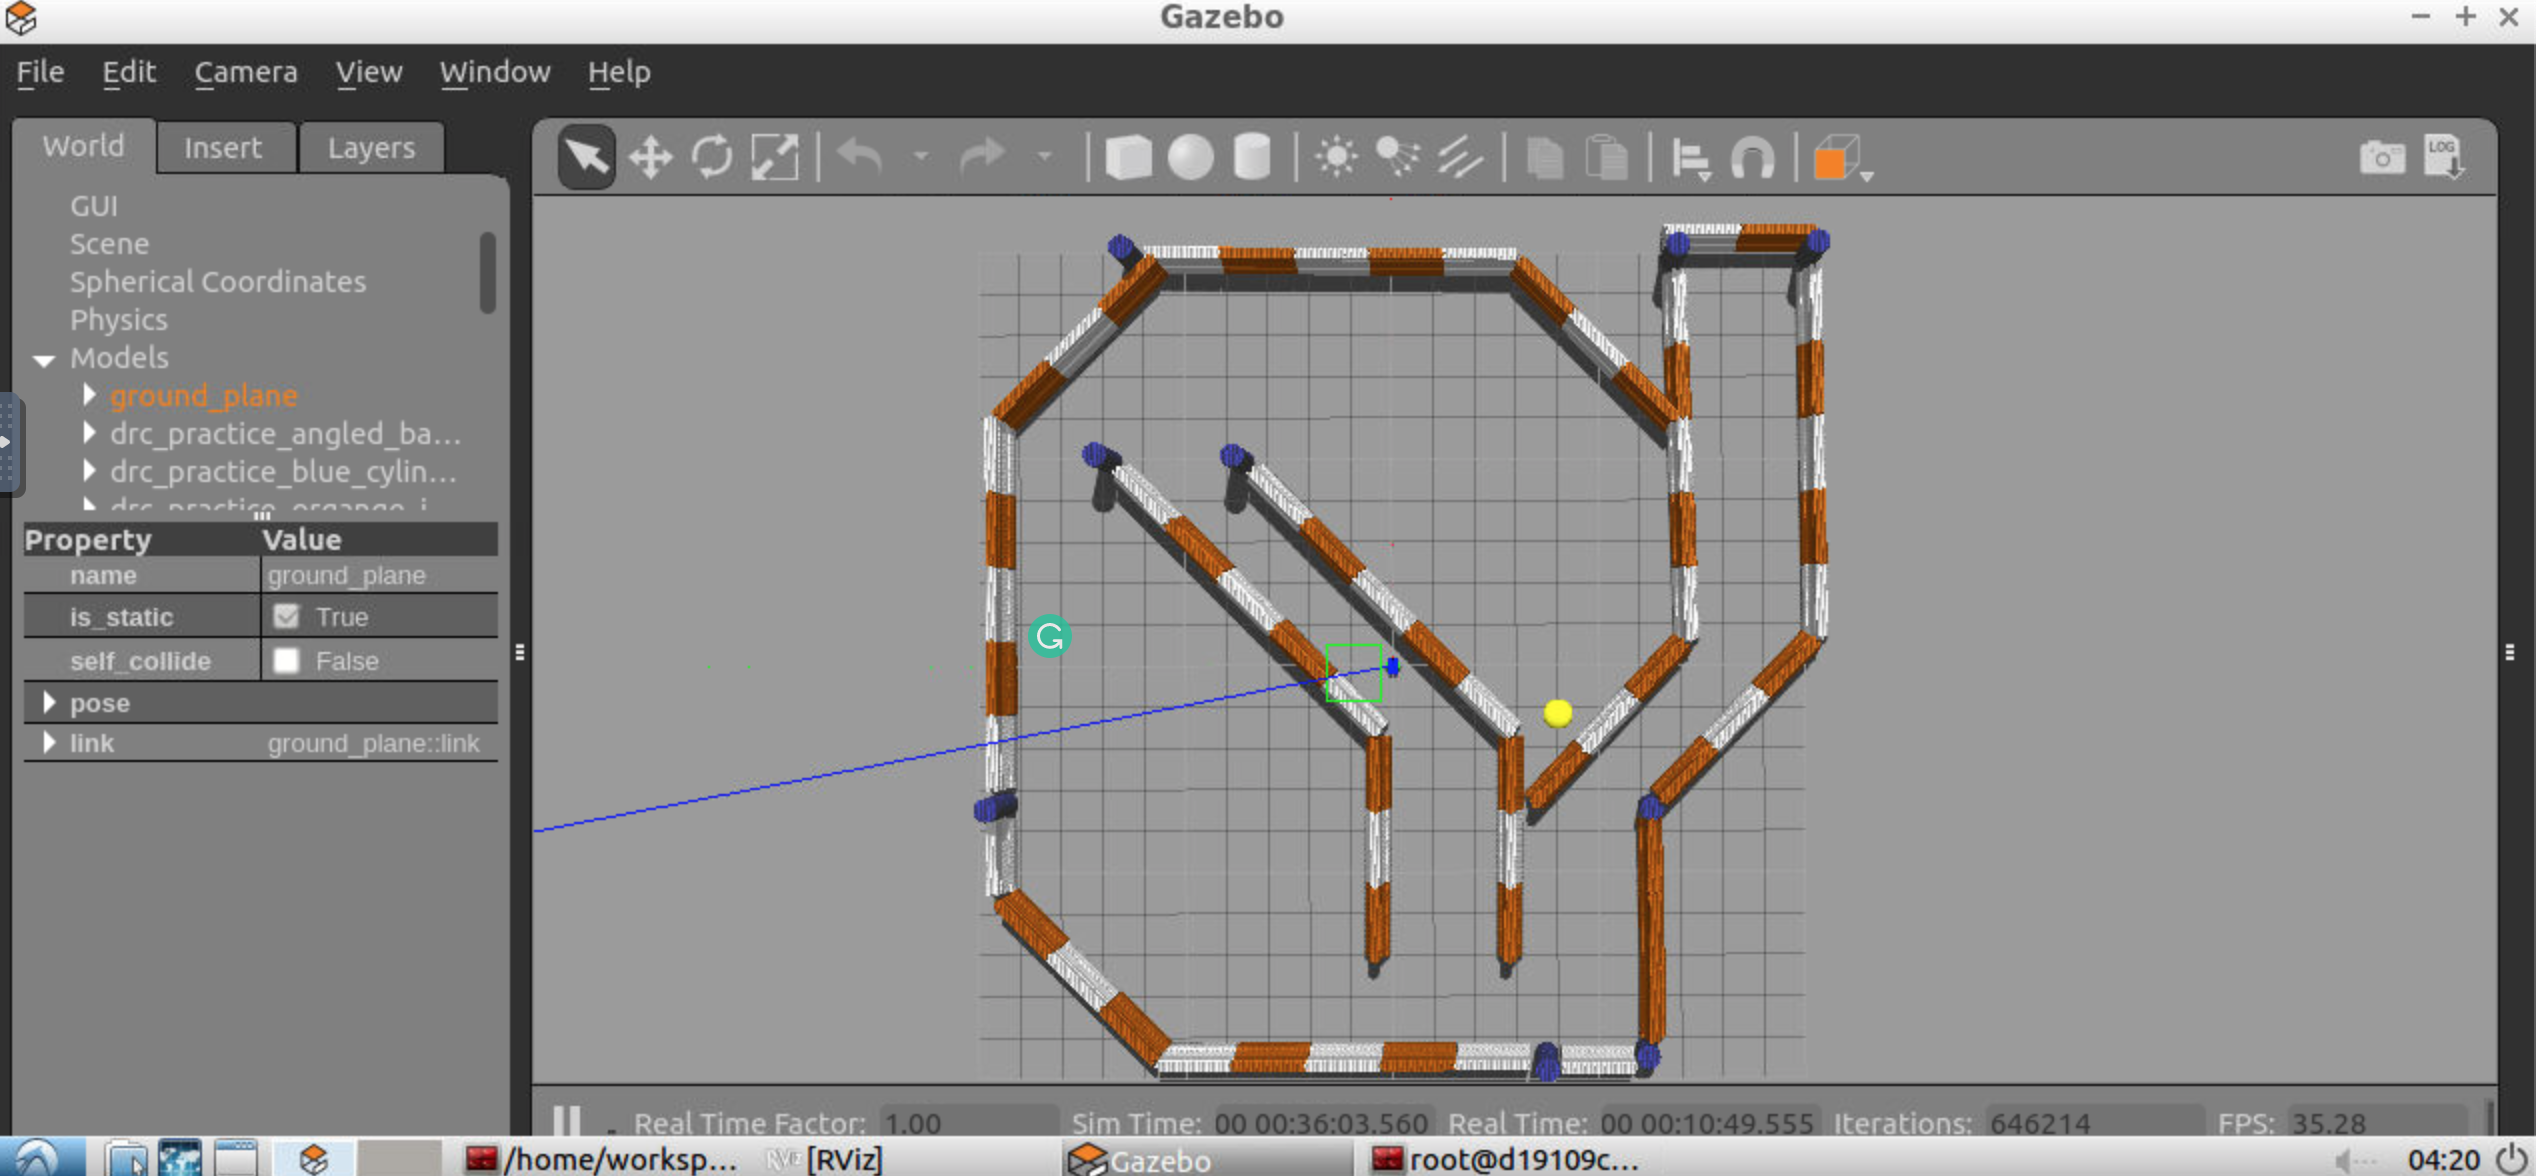
\includegraphics[width=\linewidth]{MapRobot.png}
      \caption{Robot Revolution.}
      \label{fig:robot1}
\end{figure}

\section{Background}
In the book Probabilistic Robotic (Thrun et al. 2005) described there are several approach to help robot perform localization problem from Extend Kalman filter to Marco, to Monte Carlo and finally Grid. In this project, Jackal race world is a local localization problem which has information robot's initial pose relate to static environment collecting sensory information using range finder sensors from environment.

\subsection{Kalman Filters}
 Kalman filters can take data with a lot of noisy or uncertainty in the measurements and provide very accurate estimate of the real value and can do it very fast don't need wait a lot of data to come. The Kalman Filter is applicable to problems with linear motion and measurement functions. This is limiting, as much of the real world is nonlinear.
 
\subsection{Particle Filters}
MCL can solve local and global localization problems represents non Gaussian distribution and can approximate any other practical important distribution not limited to linear model. 
\subsection{Comparison / Contrast}
MCL is easy to program compare to EKF. MCL uses particle to localize robot's pose and can approximate almost any state space distribution. MCL uses particles to localize a robot and can approximate almost any distribution. Each particle has a position and orientation by changing the number of particles control computational memory and resolution.
%example for inserting image
\begin{figure}[thpb]
      \centering
      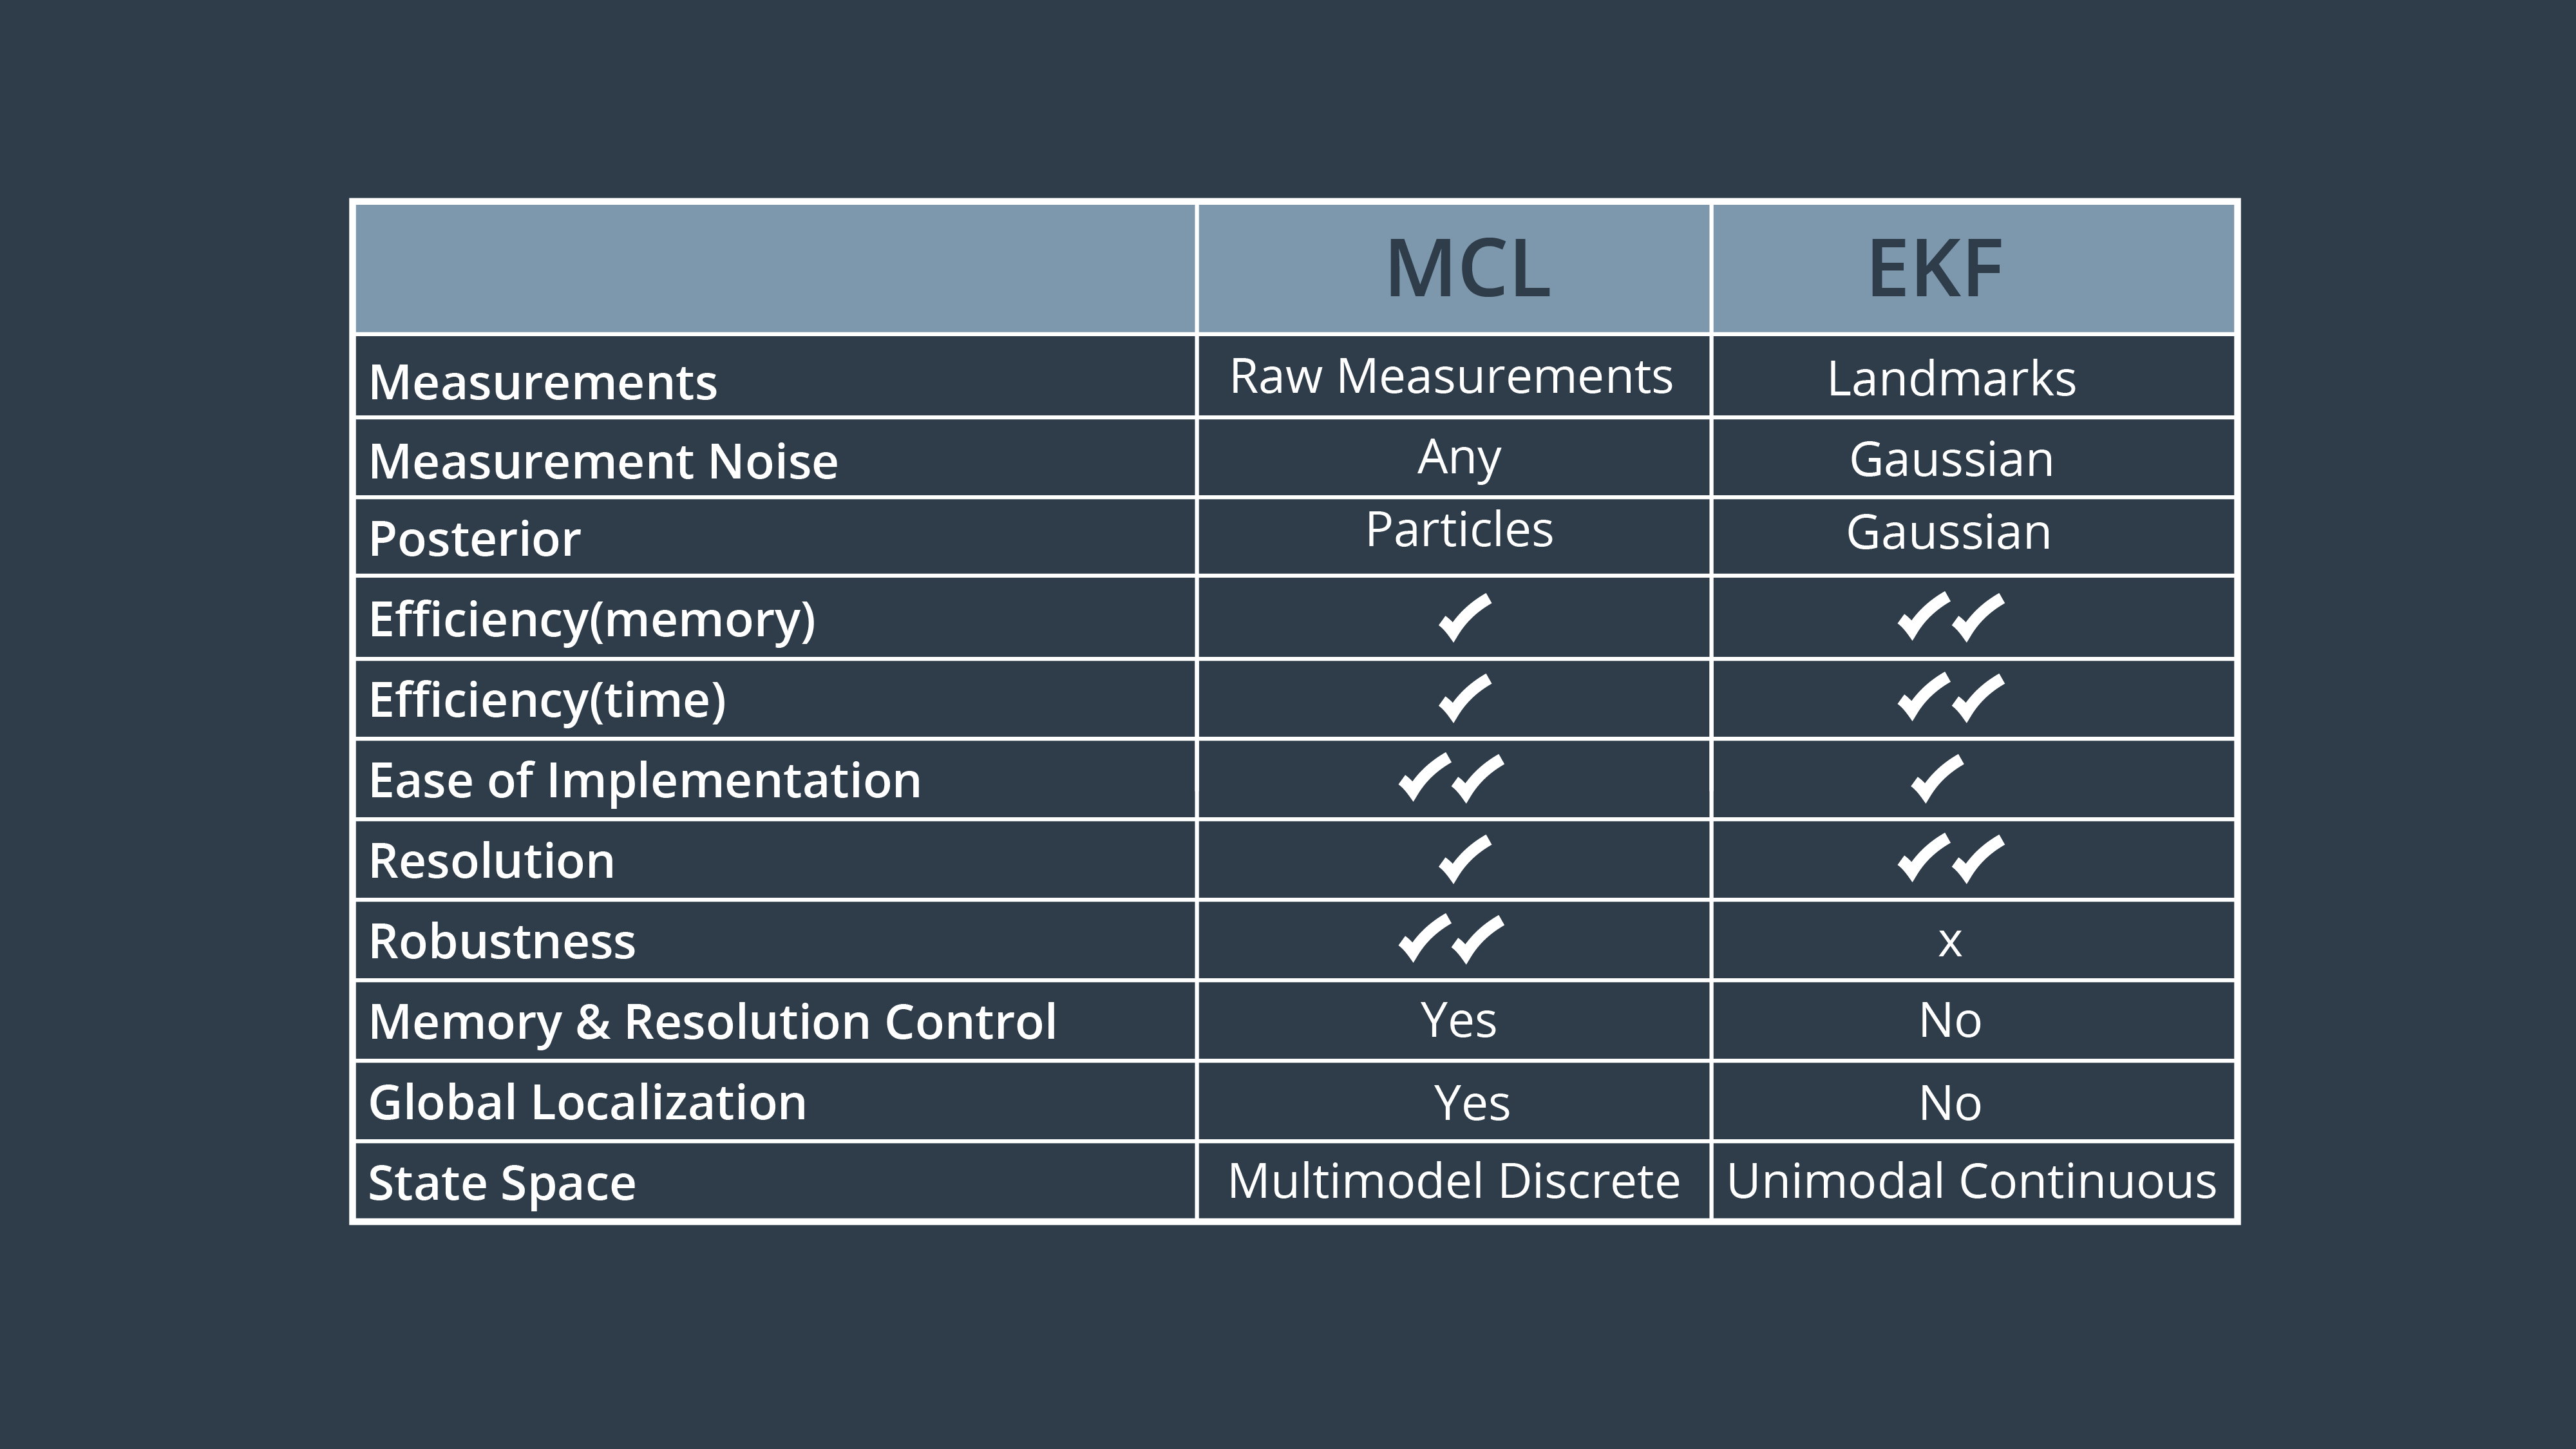
\includegraphics[width=\linewidth]{mclVsEKF.png}
      \caption{MCL VS EKF.}
      \label{fig:robot1}
\end{figure}
\section{Simulations}
 By utilize ROS packages to accurately localize a mobile robot inside a provided map in the Gazebo and RViz simulation environments. While Gazebo is a physics simulator, RViz can visualize any type of sensor data being published over a ROS topic like camera images, point clouds, Lidar data, etc. This data can be a live stream coming directly from the sensor or pre-recorded data stored as a bag file. RViz is one-stop tool to visualize all the three core aspects of a robot: Perception, Decision Making, and Actuation.  
 
 Over all ROS aspect:
\begin{itemize}
\item Building a mobile robot for simulated tasks.
\item Creating a ROS package that launches a custom robot model in a Gazebo world and utilizes packages like AMCL and the Navigation Stack.
\item Exploring, adding, and tuning specific parameters corresponding to each package to achieve the best possible localization results.
\end {itemize}

\subsection{Achievements}
By tuning parameter in costmap common params.yaml the designed robot can localized itself and reach their destination. With navigation goal.cpp node will navigation robot to It's goal.  

% Robot Models
\subsection{Benchmark Model: Udacity Bot}
\subsubsection{Model design}

%example for inserting image
\begin{figure}[thpb]
      \centering
      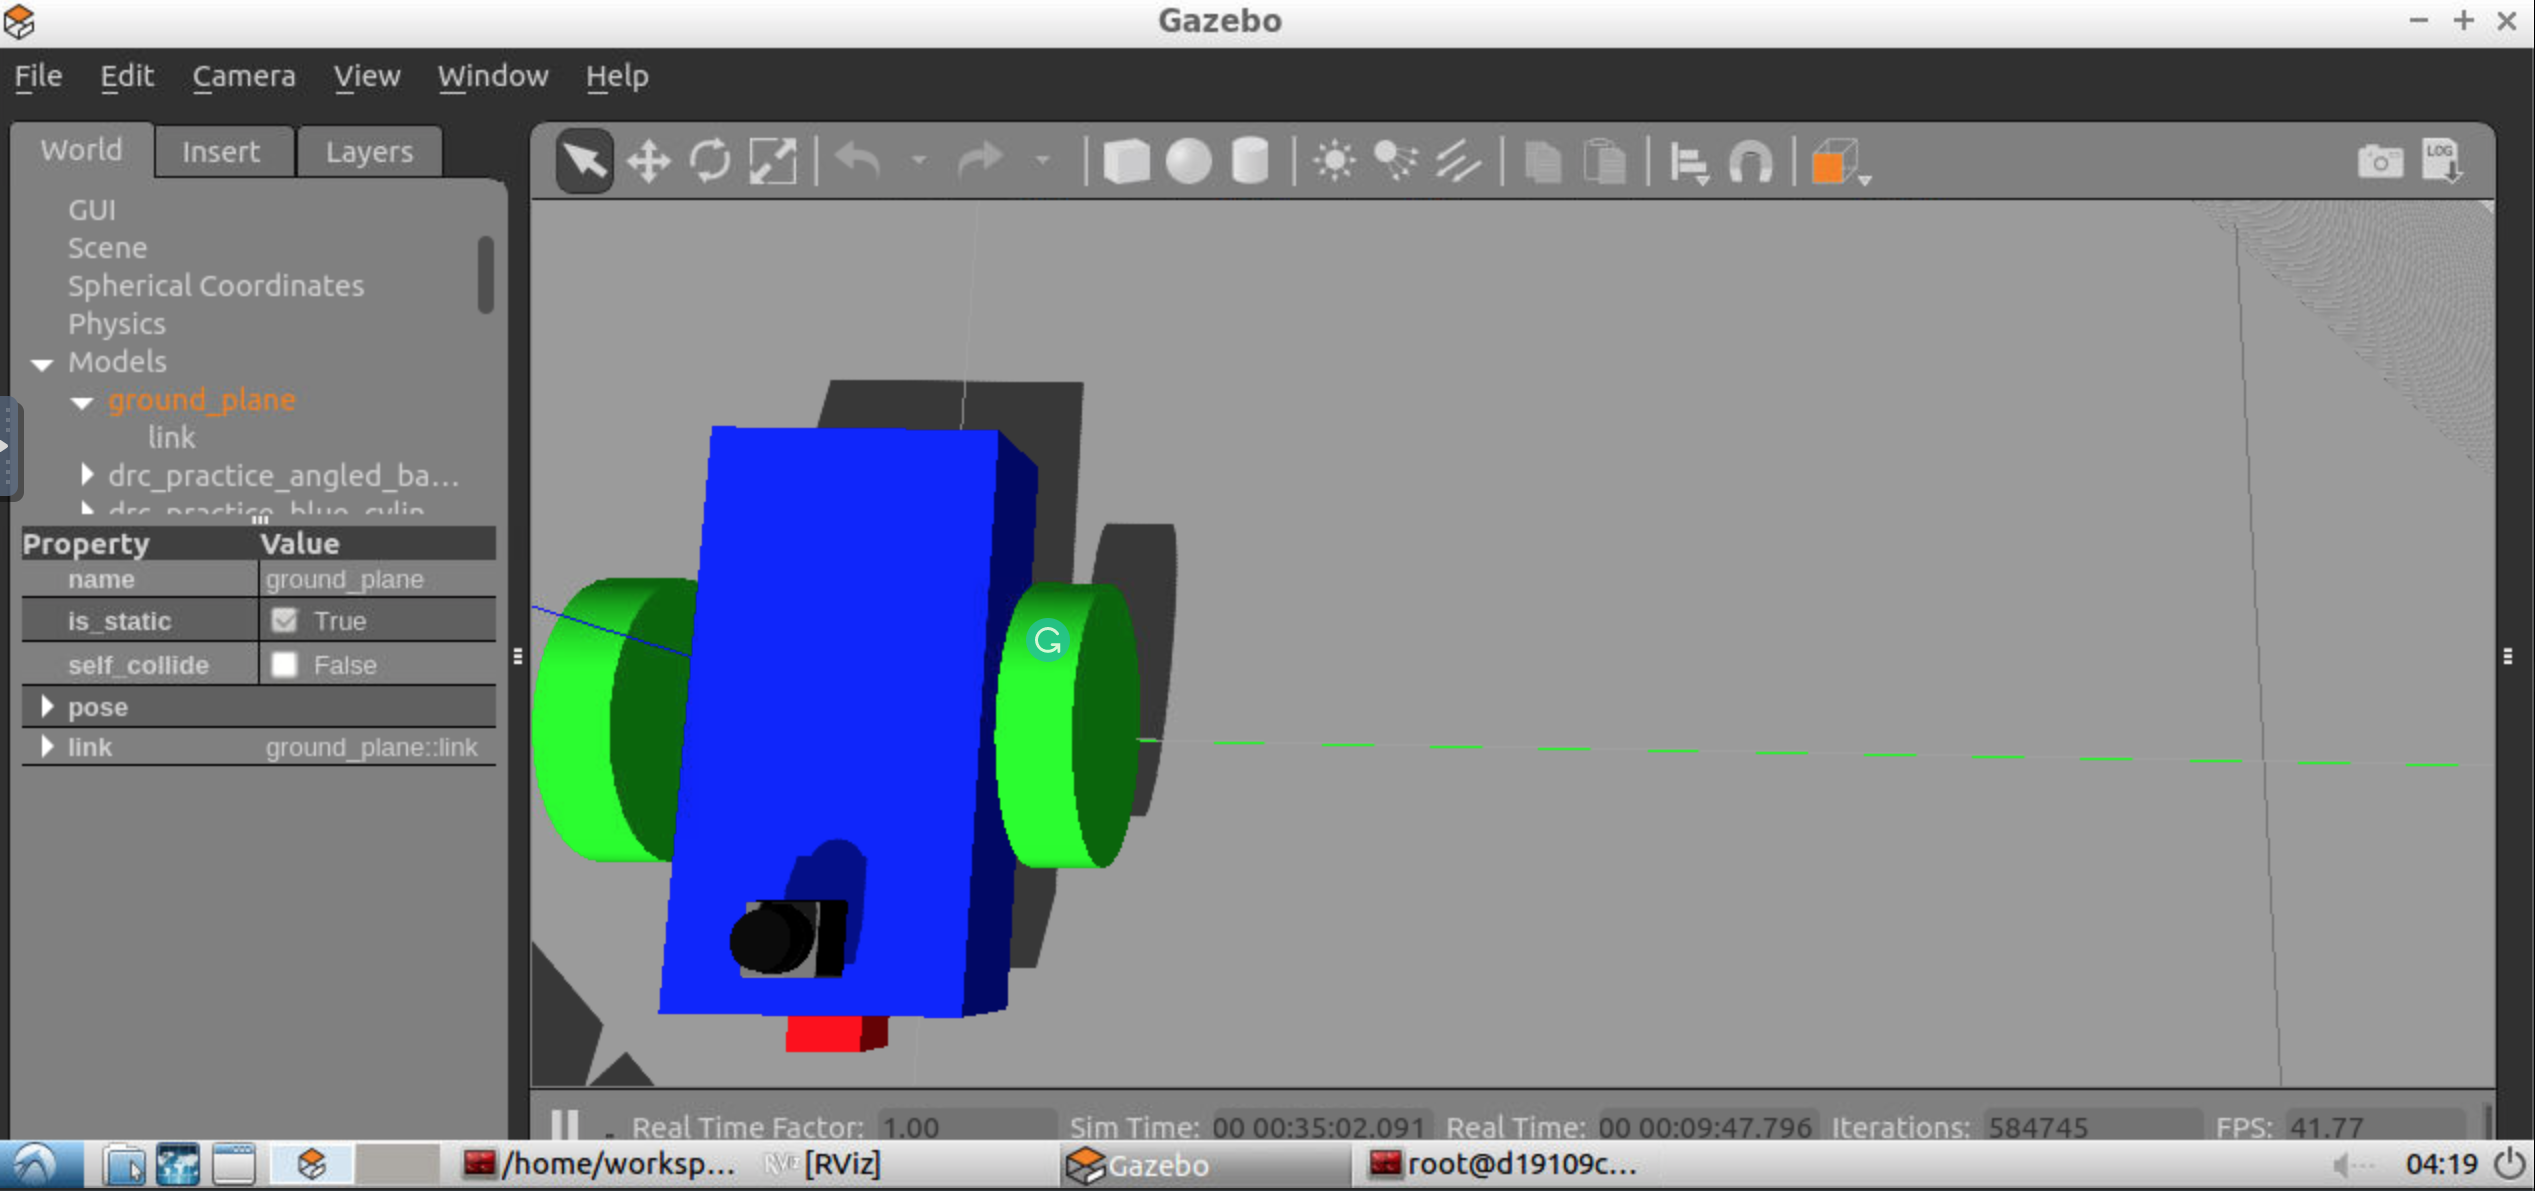
\includegraphics[width=\linewidth]{laserrangefinder.png}
      \caption{Robot model with a camera and laser rangefinder.}
      \label{fig:robot1}
\end{figure}
In this section build a very basic mobile robot model named Udacity bot by creating its Unified Robot Description Format (URDF file). The robot designed geometry and parameters such as collision and inertia are set in configure. The Udacity bot has  chassis size [0.4, 0.2, 0.1] with 2 casters provide balance with radius shape 0.0499 and two wheels with cylinder radius="0.1" length="0.05" on-board with camera and laser range finder.

\begin{table}[h]
 \begin{center}
      \begin{tabular}{ |c|c|c| } 
       \hline
       Part & Geometry & size \\
       \hline
       Left and right wheel & Cylinder & length:0.05, radius:0.1 \\
       Chassis & Cube & 0.4x0.2x0.1  \\ 
       Back and Front casters & Sphere & radius:0.0499 \\
       Camera & box & 0.05 x 0.05 x 0.05 \\
       \hline
      \end{tabular}
      \caption{Udacity bot specifications}
      \label{table:1}
      \end{center}
      \end{table}
\subsubsection{Packages Used}
In Robotics navigation, AMCL package and the Navigation stack package are crucial for localize and navigation robot. AMCL package can dynamically adjusts the number of particles over a period of time, as the robot navigates around in a map. This adaptive process offers a significant computational advantage over MCL.  

Udacity Bot package
\begin{itemize}
\item config
\item launch
\item maps
\item meshes
\item src
\item urdf
\item worlds
\item rviz
\end {itemize}
\subsubsection{Parameters}
Localization parameters in the AMCL node such as min and max particles is crucial as we can set from 10 to 100 to observe the performance and memory usage. As the particles increase same as the accuracy will increase. By tuning transform tolerance parameter will fix Costmap2DROS transform timeout indicative of the maximum allowed delay to either be not defined or to be too low for the system to compensate for. This maximum amount of delay or latency allowed between transforms is defined by the transform tolerance parameter. Except transform tolerance parameter several parameter was tested and tuned such as obstacle range, raytrace range and inflation radius. By increasing inflation radius will influence obstacles detect and the obstacles distance between the robot.
\begin{table}[h]
 \begin{center}
       Costmap Parameters \\
       \hline
      \begin{tabular}{ |c|c|c| } 
       Parameter & Global & local \\
       \hline
       global frame & map & Odom \\
       robot base frame & robot footprint & robot footprint  \\ 
       update frequency & 50.0 & 50.0 \\
       publish frequency & 50.0 & 50.0\\
       width & 40.0 & 20.0\\
       height & 40.0 & 20.0 \\
       resolution & 0.05  & 0.05 \\
       static map & true & false \\
       rolling window & false & true\\
       \hline
      \end{tabular}
      \caption{Udacity bot specifications}
      \label{table:1}
      \end{center}
      \end{table}

\begin{table}[h]
 \begin{center}
       AMCL node Parameters\\
      \begin{tabular}{ |c|c| } 
       min particles & 100 \\
       \hline
       max particles & 5000 \\
       \hline
       laser max beams & 30 \\
       \hline
      \end{tabular}
      \caption{Udacity bot specifications}
      \label{table:1}
      \end{center}
      \end{table}
\subsection{Personal Model}
% ditto
\subsubsection{Model design}
By creating another Robot Description Format (URDF file) base on Udacity bot and the same package to perform publisher and subscriber .The designed a robot model named Hsin bot has chassis size [0.4, 0.2, 0.1] with 2 casters provide balance with radius shape 0.0499 and two wheels with cylinder radius="0.1" length="0.05" on-board with camera and laser range finder which the camera is mount on front chassis has size [0.05,0.05, 0.05] and add three long and short back shield with size [0.1, 0.02, 0.12] and [0.1, 0.3, 0.02]. 
%example for inserting image
\begin{figure}[thpb]
      \centering
      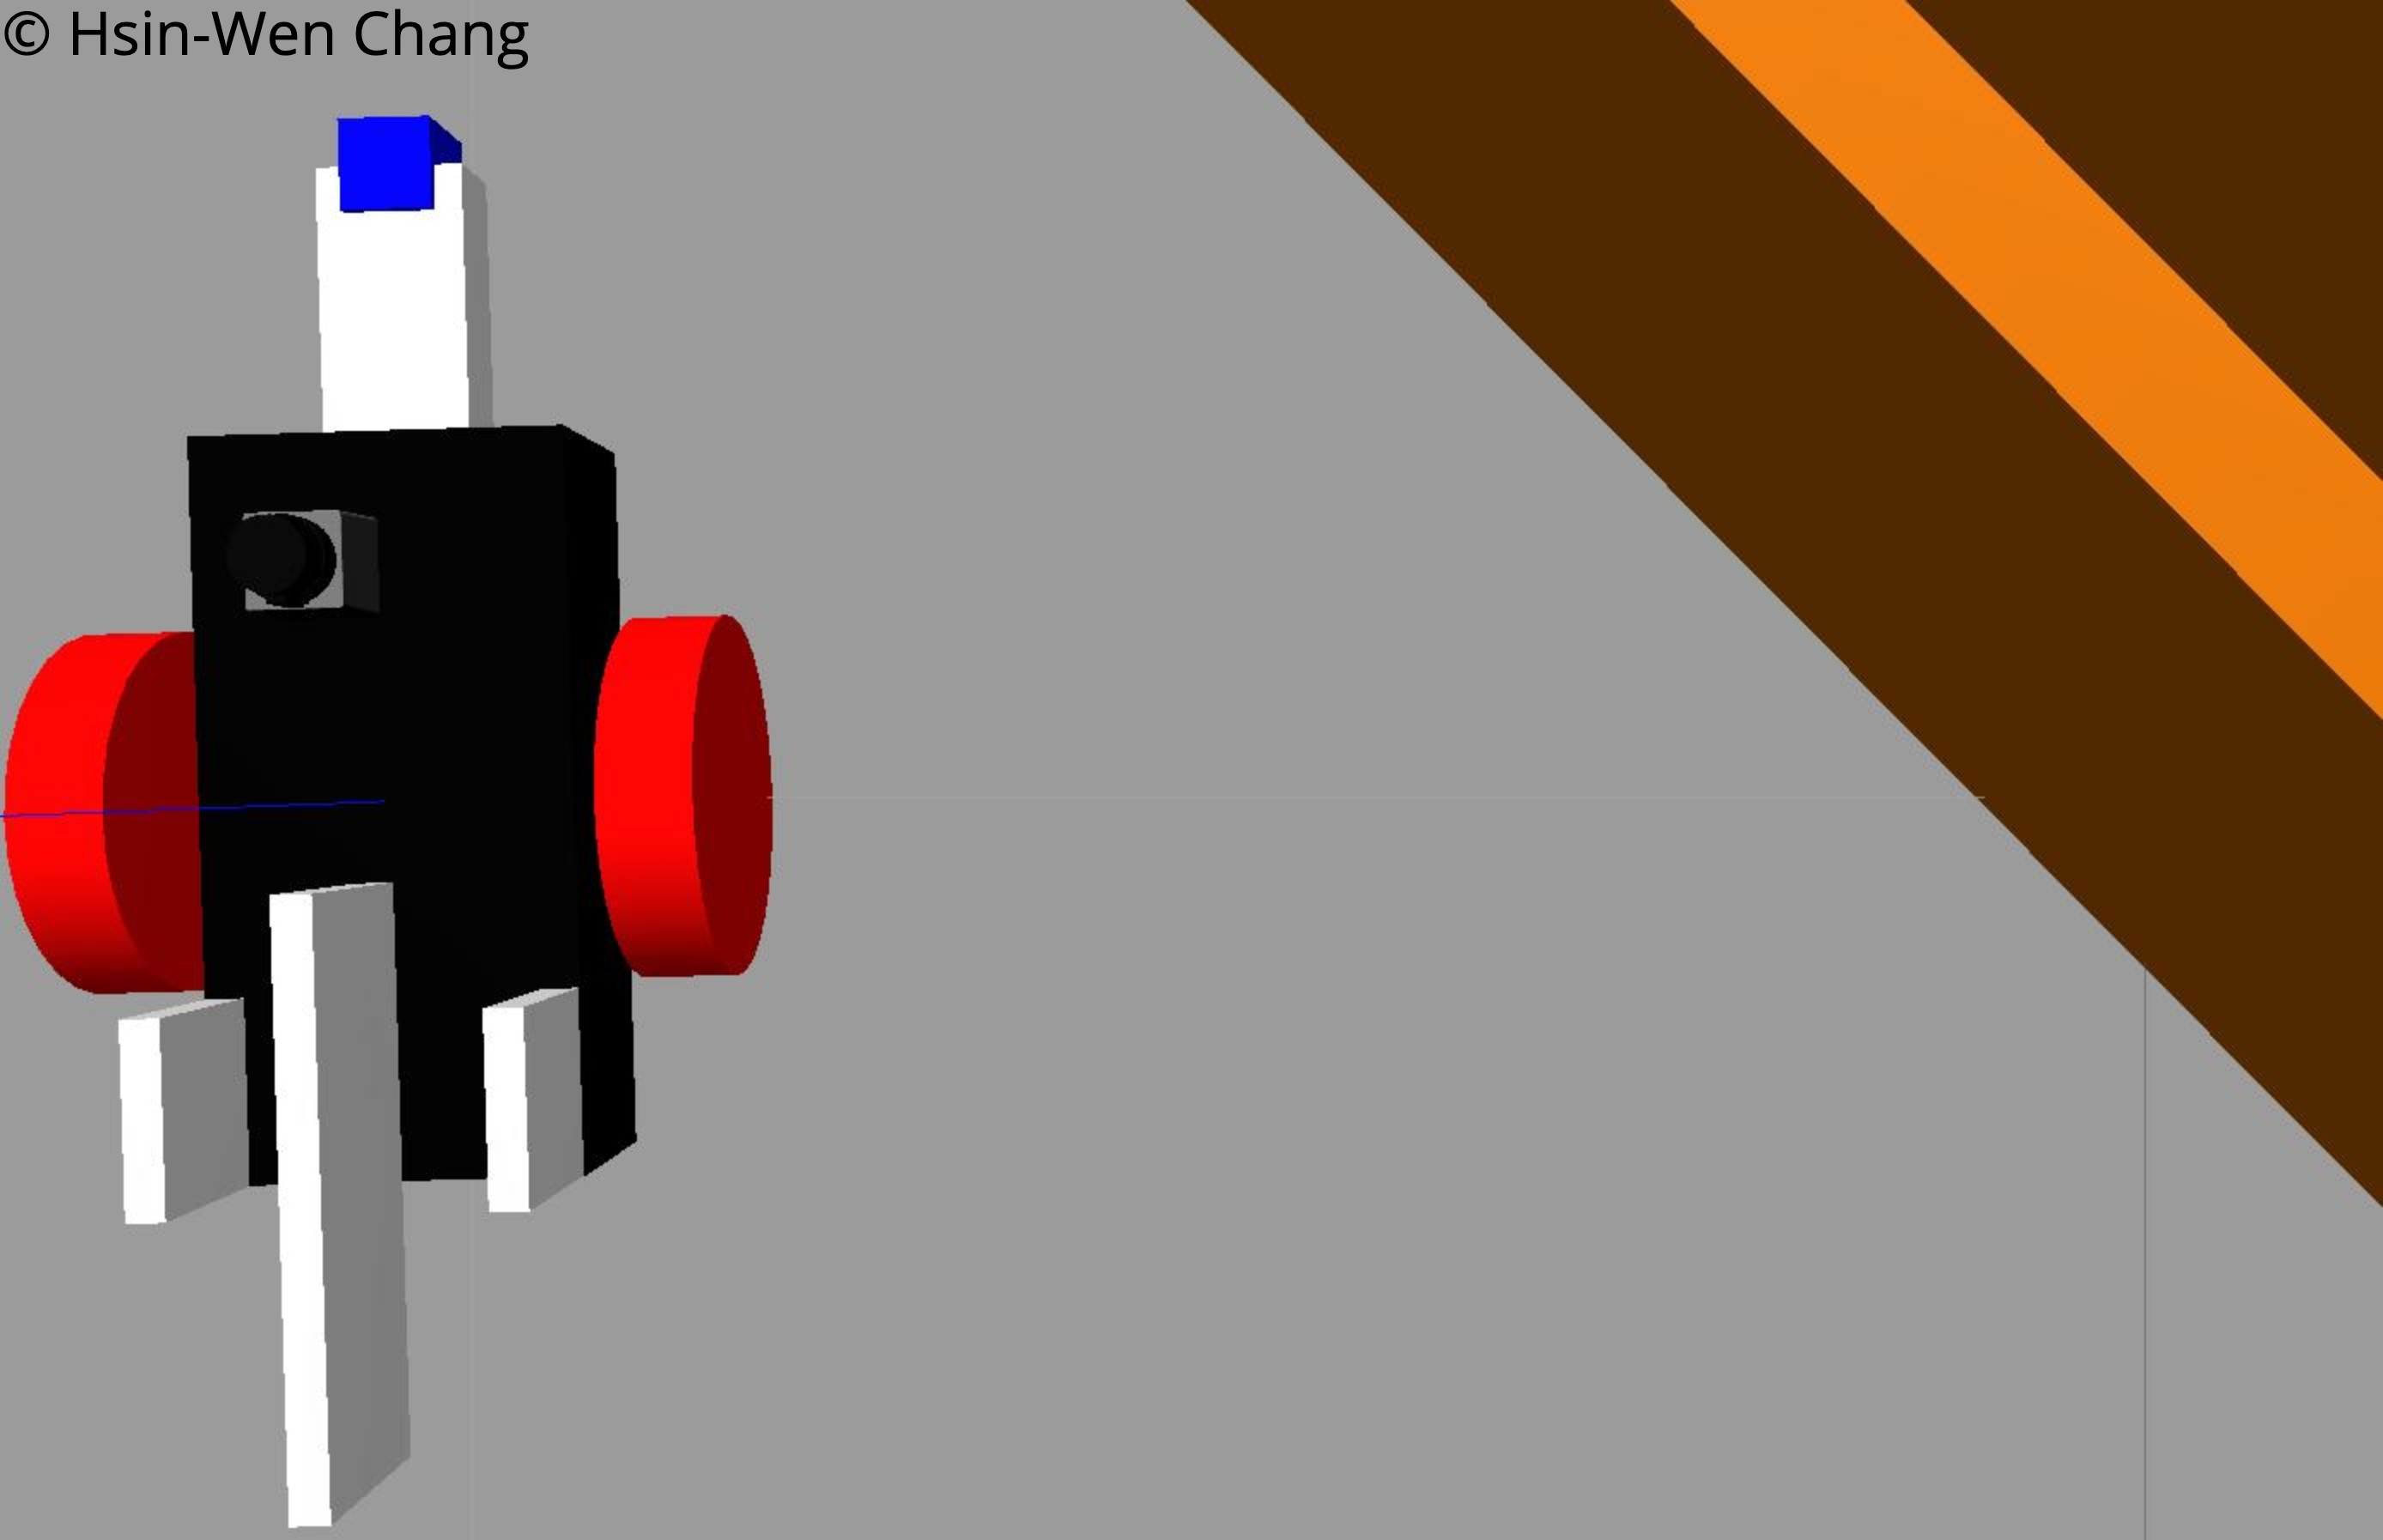
\includegraphics[width=\linewidth]{HsinBot1.jpg}
      \caption{Hsin bot right front.}
      \label{fig:robot1}
\end{figure}
%example for inserting image
\begin{figure}[thpb]
      \centering
      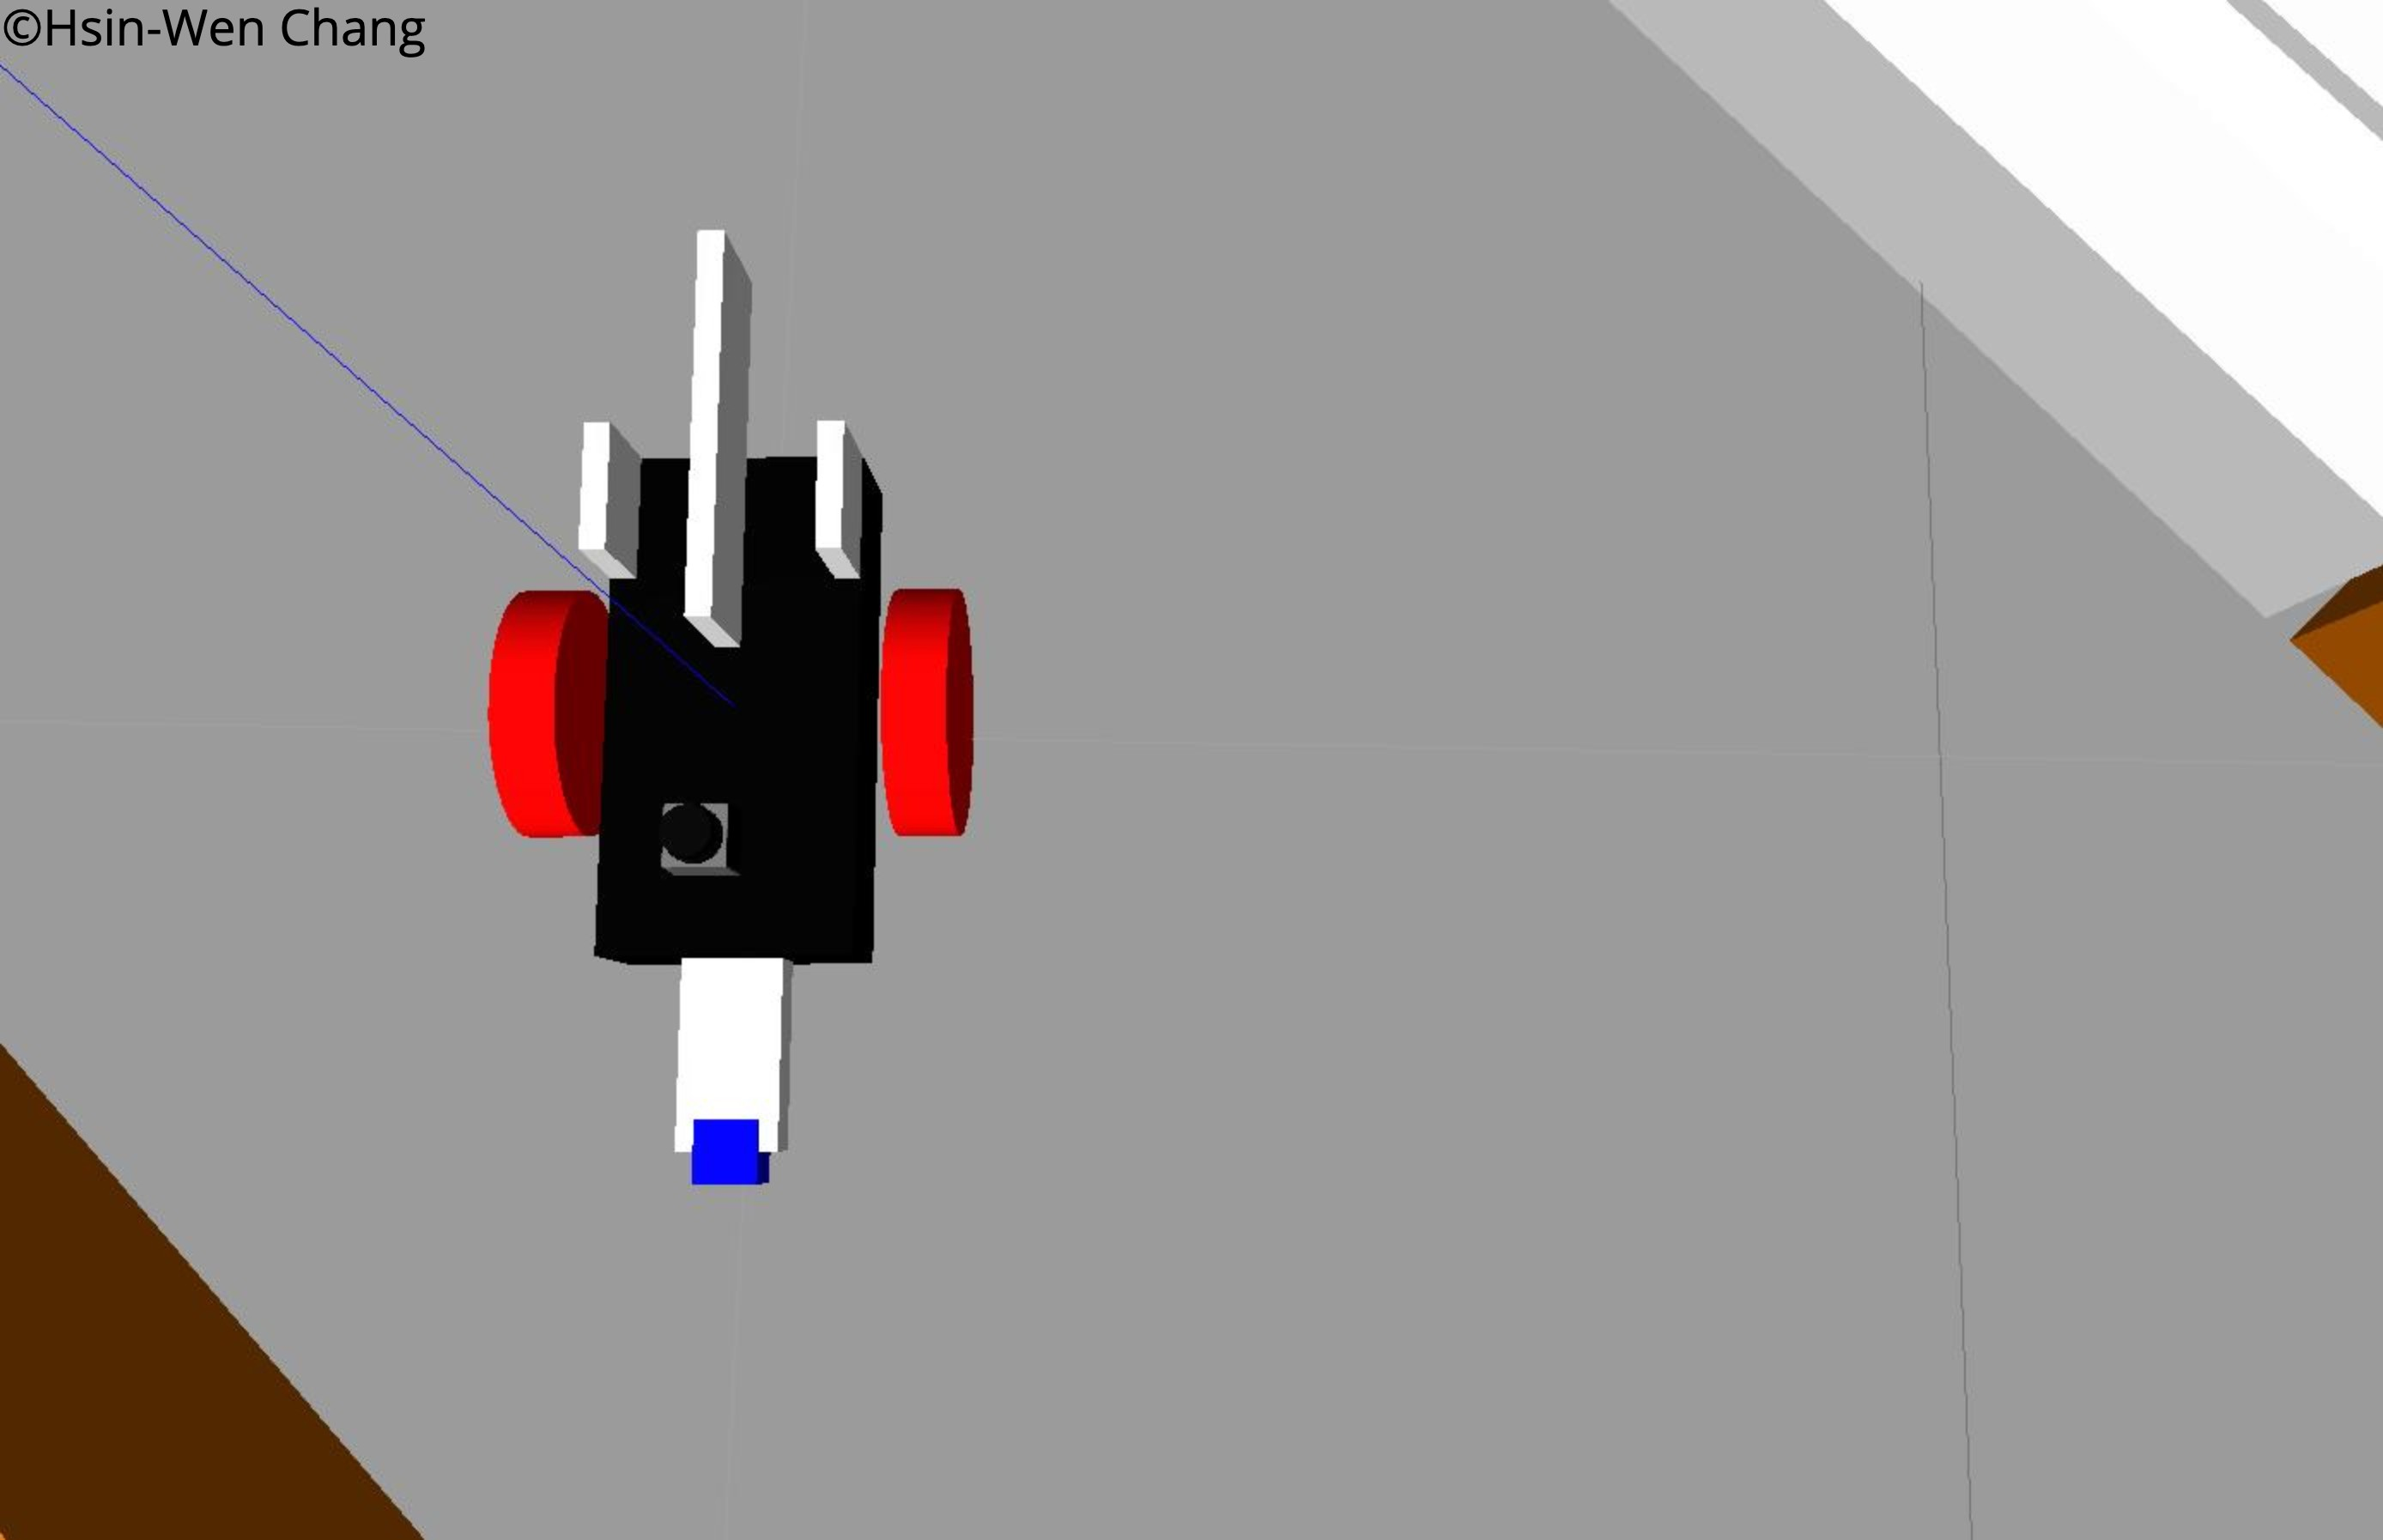
\includegraphics[width=\linewidth]{HsinBot2.jpg}
      \caption{Hsin bot top front.}
      \label{fig:robot1}
\end{figure}
\subsubsection{Packages Used}
HsinBot package
\begin{itemize}
\item config
\item launch
\item maps
\item meshes
\item src
\item urdf
\item worlds
\item rviz
\end {itemize}
\subsubsection{Parameters}
Most of the configuration of parameters in Hsin bot is base on Udacity bot except laser max beams to 20 in each scan to be used when updating the filter. Minimum allowed 50 number of particles. Maximum allowed 200 number of particles.
\begin{table}[h]
 \begin{center}
      \begin{tabular}{ |c|c|c| } 
       \hline
       Part & Geometry & size \\
       \hline
       Left and right wheel & Cylinder & length:0.05, radius:0.1 \\
       Chassis & Cube & 0.4x0.2x0.1  \\ 
       Camera & box & 0.05 x 0.05 x 0.05 \\
       Back and Front casters & Sphere & radius:0.0499 \\
       Back shield1 & box & 0.1 x 0.3 x 0.02 \\
       Left Back shield & box & 0.1 x 0.02 x 0.12 \\
       Right Back shield & box & 0.1 x 0.02 x 0.12 \\
       \hline
      \end{tabular}
      \caption{Hsin bot specifications}
      \label{table:1}
      \end{center}
      \end{table}
\begin{table}[h]
 \begin{center}
       Costmap Parameters \\
       \hline
      \begin{tabular}{ |c|c|c| } 
       Parameter & Global & local \\
       \hline
       global frame & map & Odom \\
       robot base frame & robot footprint & robot footprint  \\ 
       update frequency & 50.0 & 50.0 \\
       publish frequency & 50.0 & 50.0\\
       width & 40.0 & 20.0\\
       height & 40.0 & 20.0 \\
       resolution & 0.05  & 0.05 \\
       static map & true & false \\
       rolling window & false & true\\
       \hline
      \end{tabular}
      \caption{Hsin bot specifications}
      \label{table:1}
      \end{center}
      \end{table}
\begin{table}[h]
 \begin{center}
       AMCL node Parameters\\
      \begin{tabular}{ |c|c| } 
       min particles & 50 \\
       \hline
       max particles & 200 \\
       \hline
       laser max beams & 20 \\
       \hline
      \end{tabular}
      \caption{Hsin bot specifications}
      \label{table:1}
      \end{center}
      \end{table}
\begin{table}[h]
 \begin{center}
 costmap common params\\
      \hline
      \begin{tabular}{ |c|c| }
       obstacle range & 1.2 \\
       \hline
       raytrace range & 1.2 \\
       \hline
       inflation radius & 0.4 \\
       \hline
       observation sources & laser scan sensor \\
       \hline
      \end{tabular}
      \caption{Hsin bot specifications}
      \label{table:1}
      \end{center}
      \end{table}  
    
\section{Results}
After parameter tuning and testing both robots are able to reach their destination

\subsection{Localization Results}
\subsubsection{Benchmark}
%example for inserting image
\begin{figure}[thpb]
      \centering
      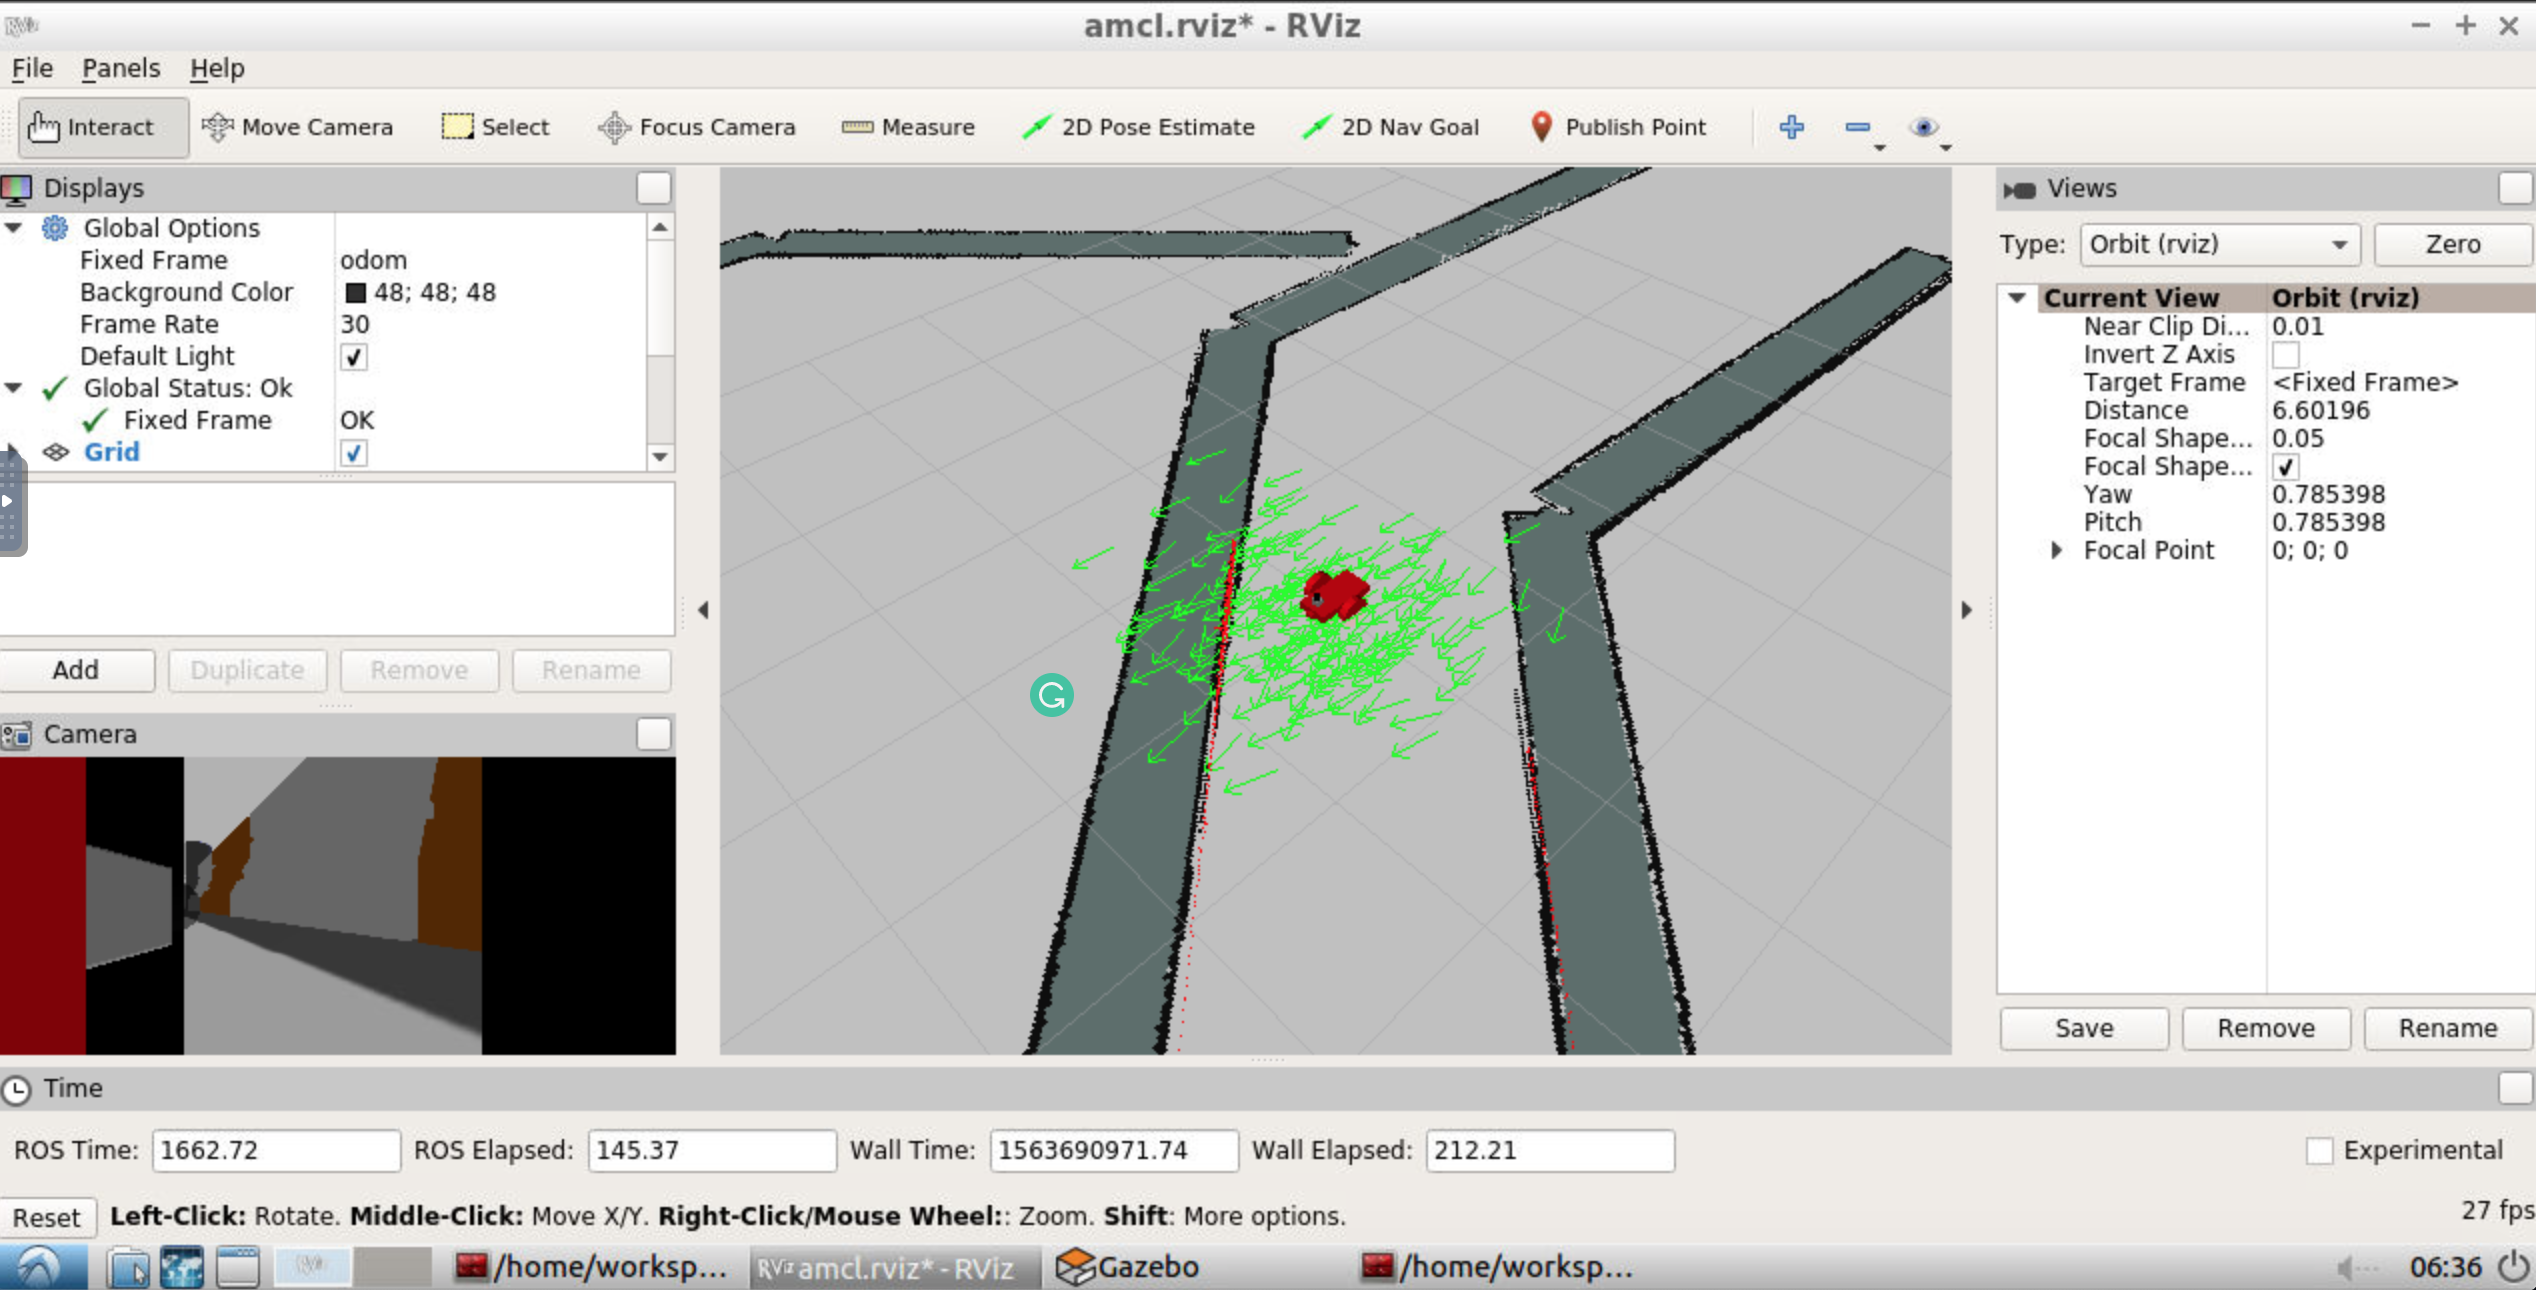
\includegraphics[width=\linewidth]{acml.png}
      \caption{Udacity bot model with a camera and laser rangefinder.}
      \label{fig:robot1}
\end{figure}
%example for inserting image
\begin{figure}[thpb]
      \centering
      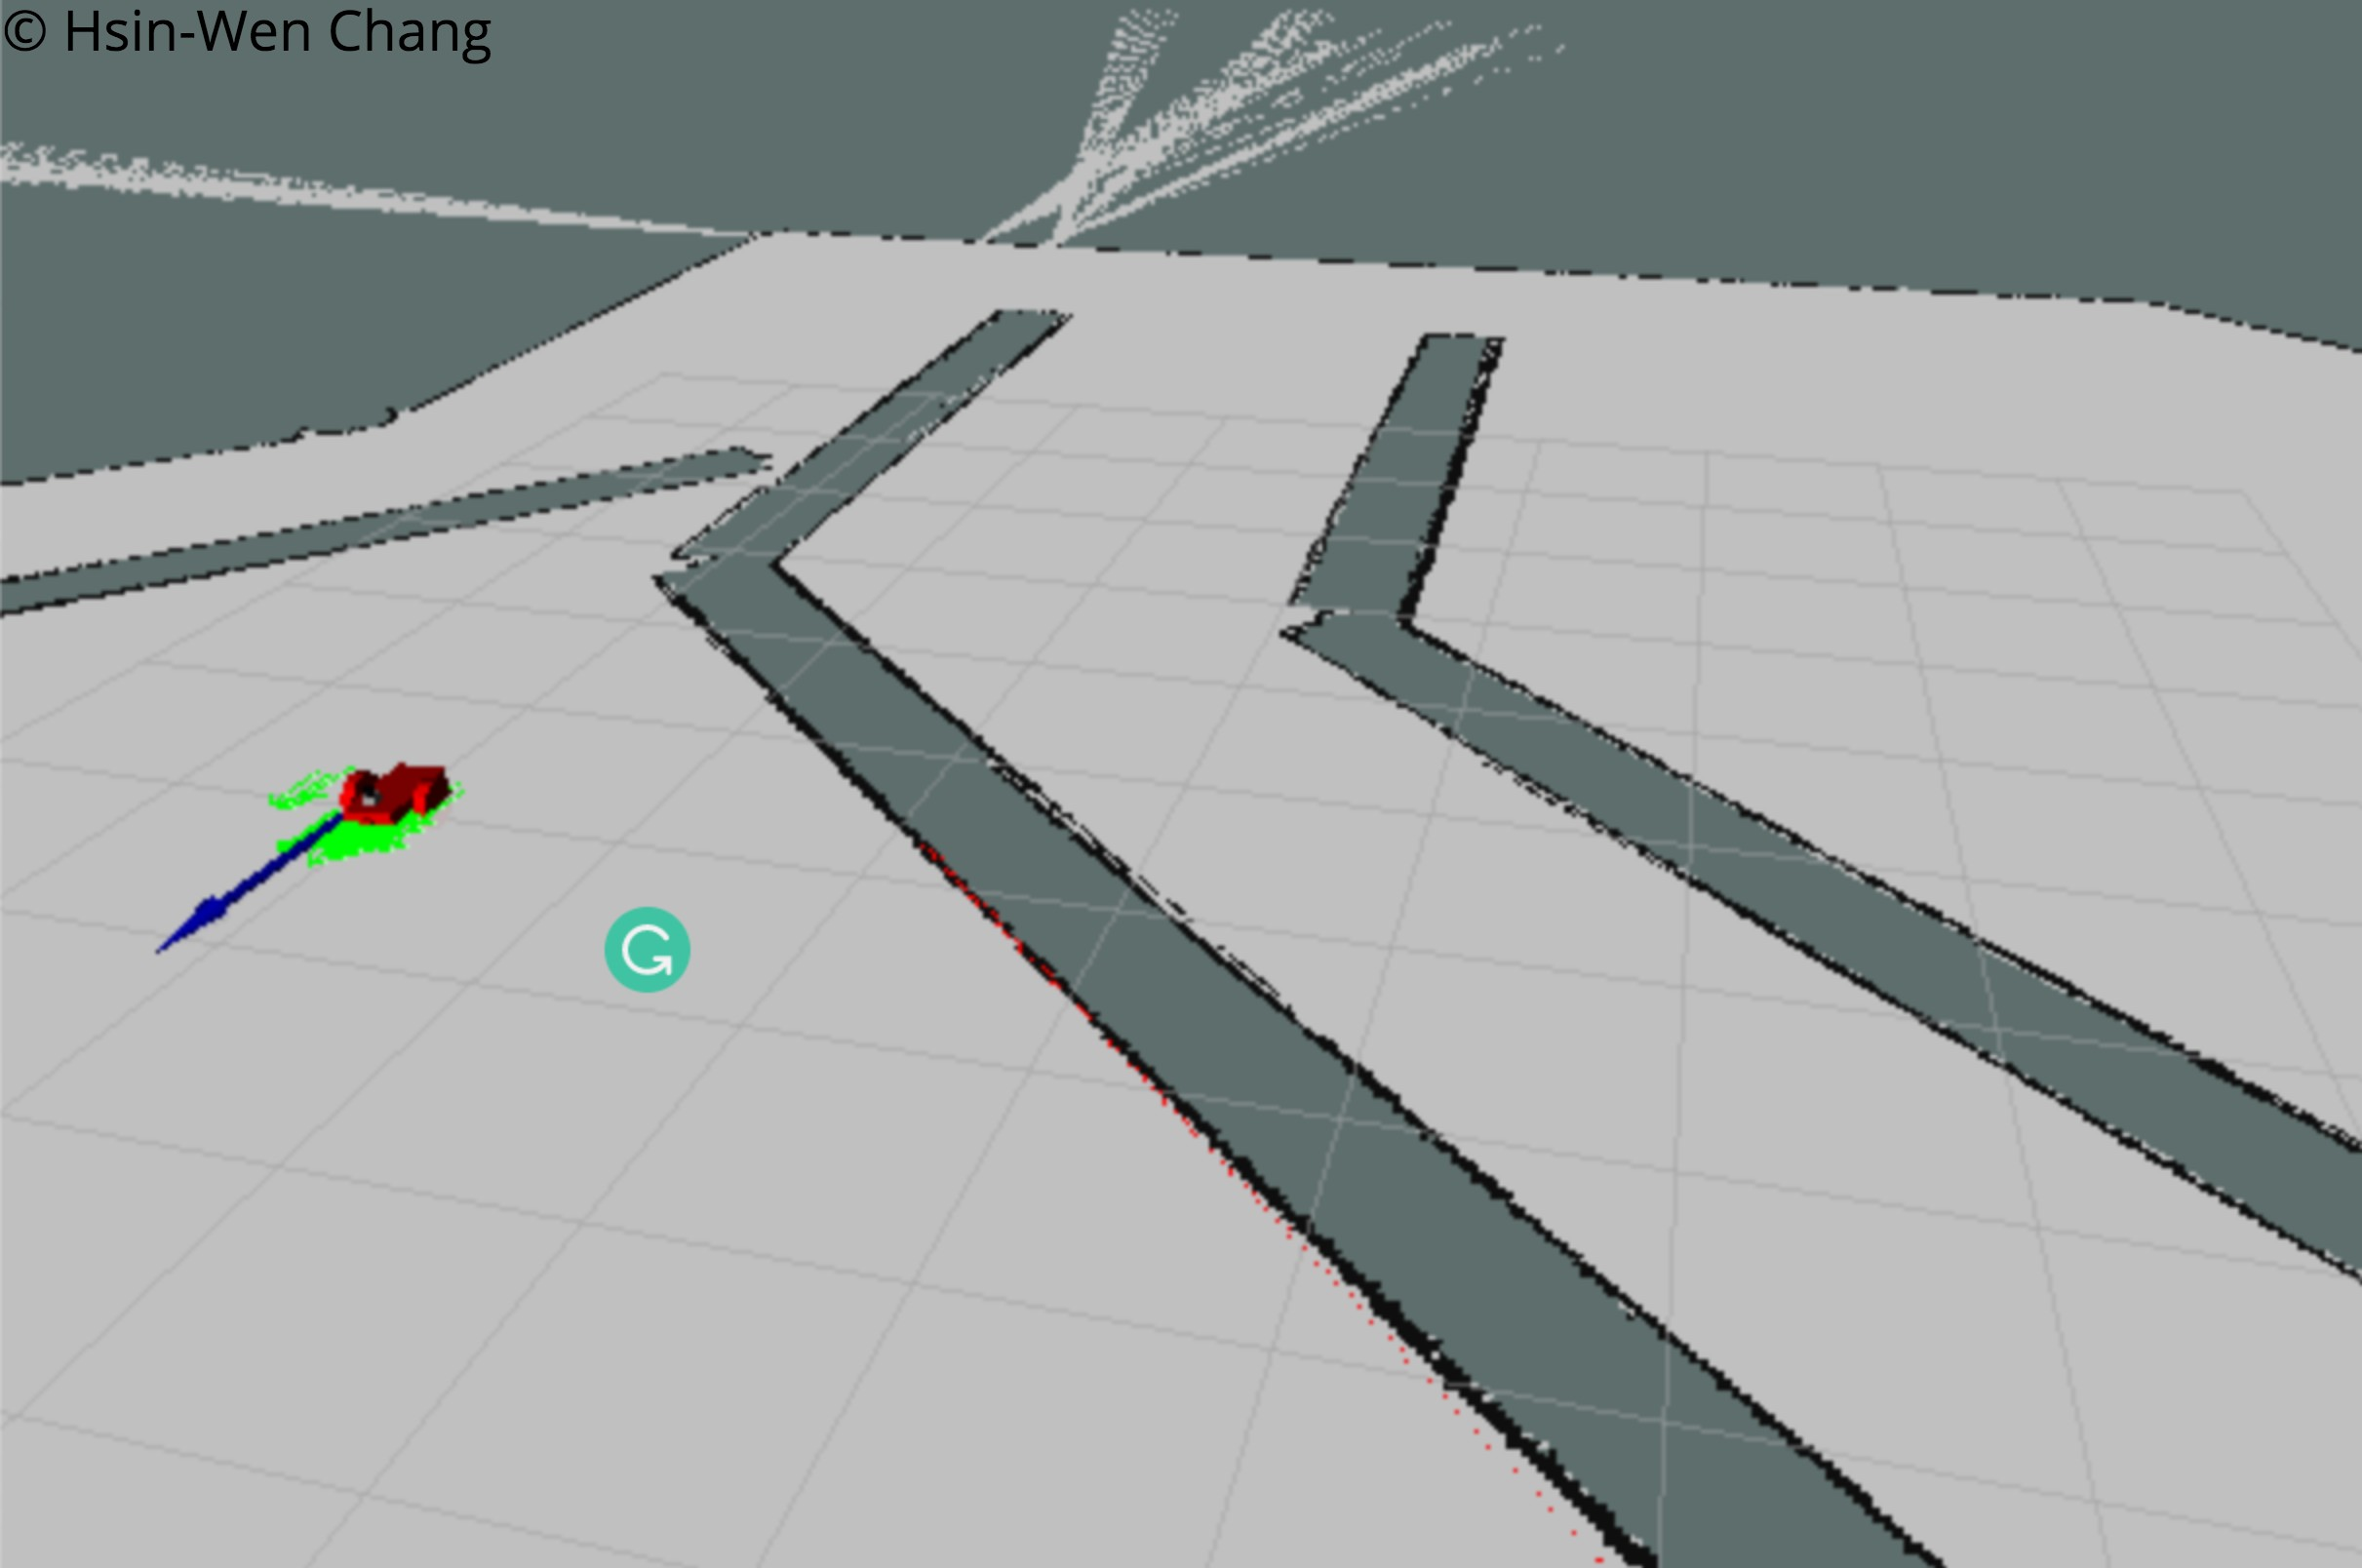
\includegraphics[width=\linewidth]{f2.png}
      \caption{Udacity bot reaching the goal position.}
      \label{fig:robot1}
\end{figure}
\subsubsection{Student}
%example for inserting image
\begin{figure}[thpb]
      \centering
      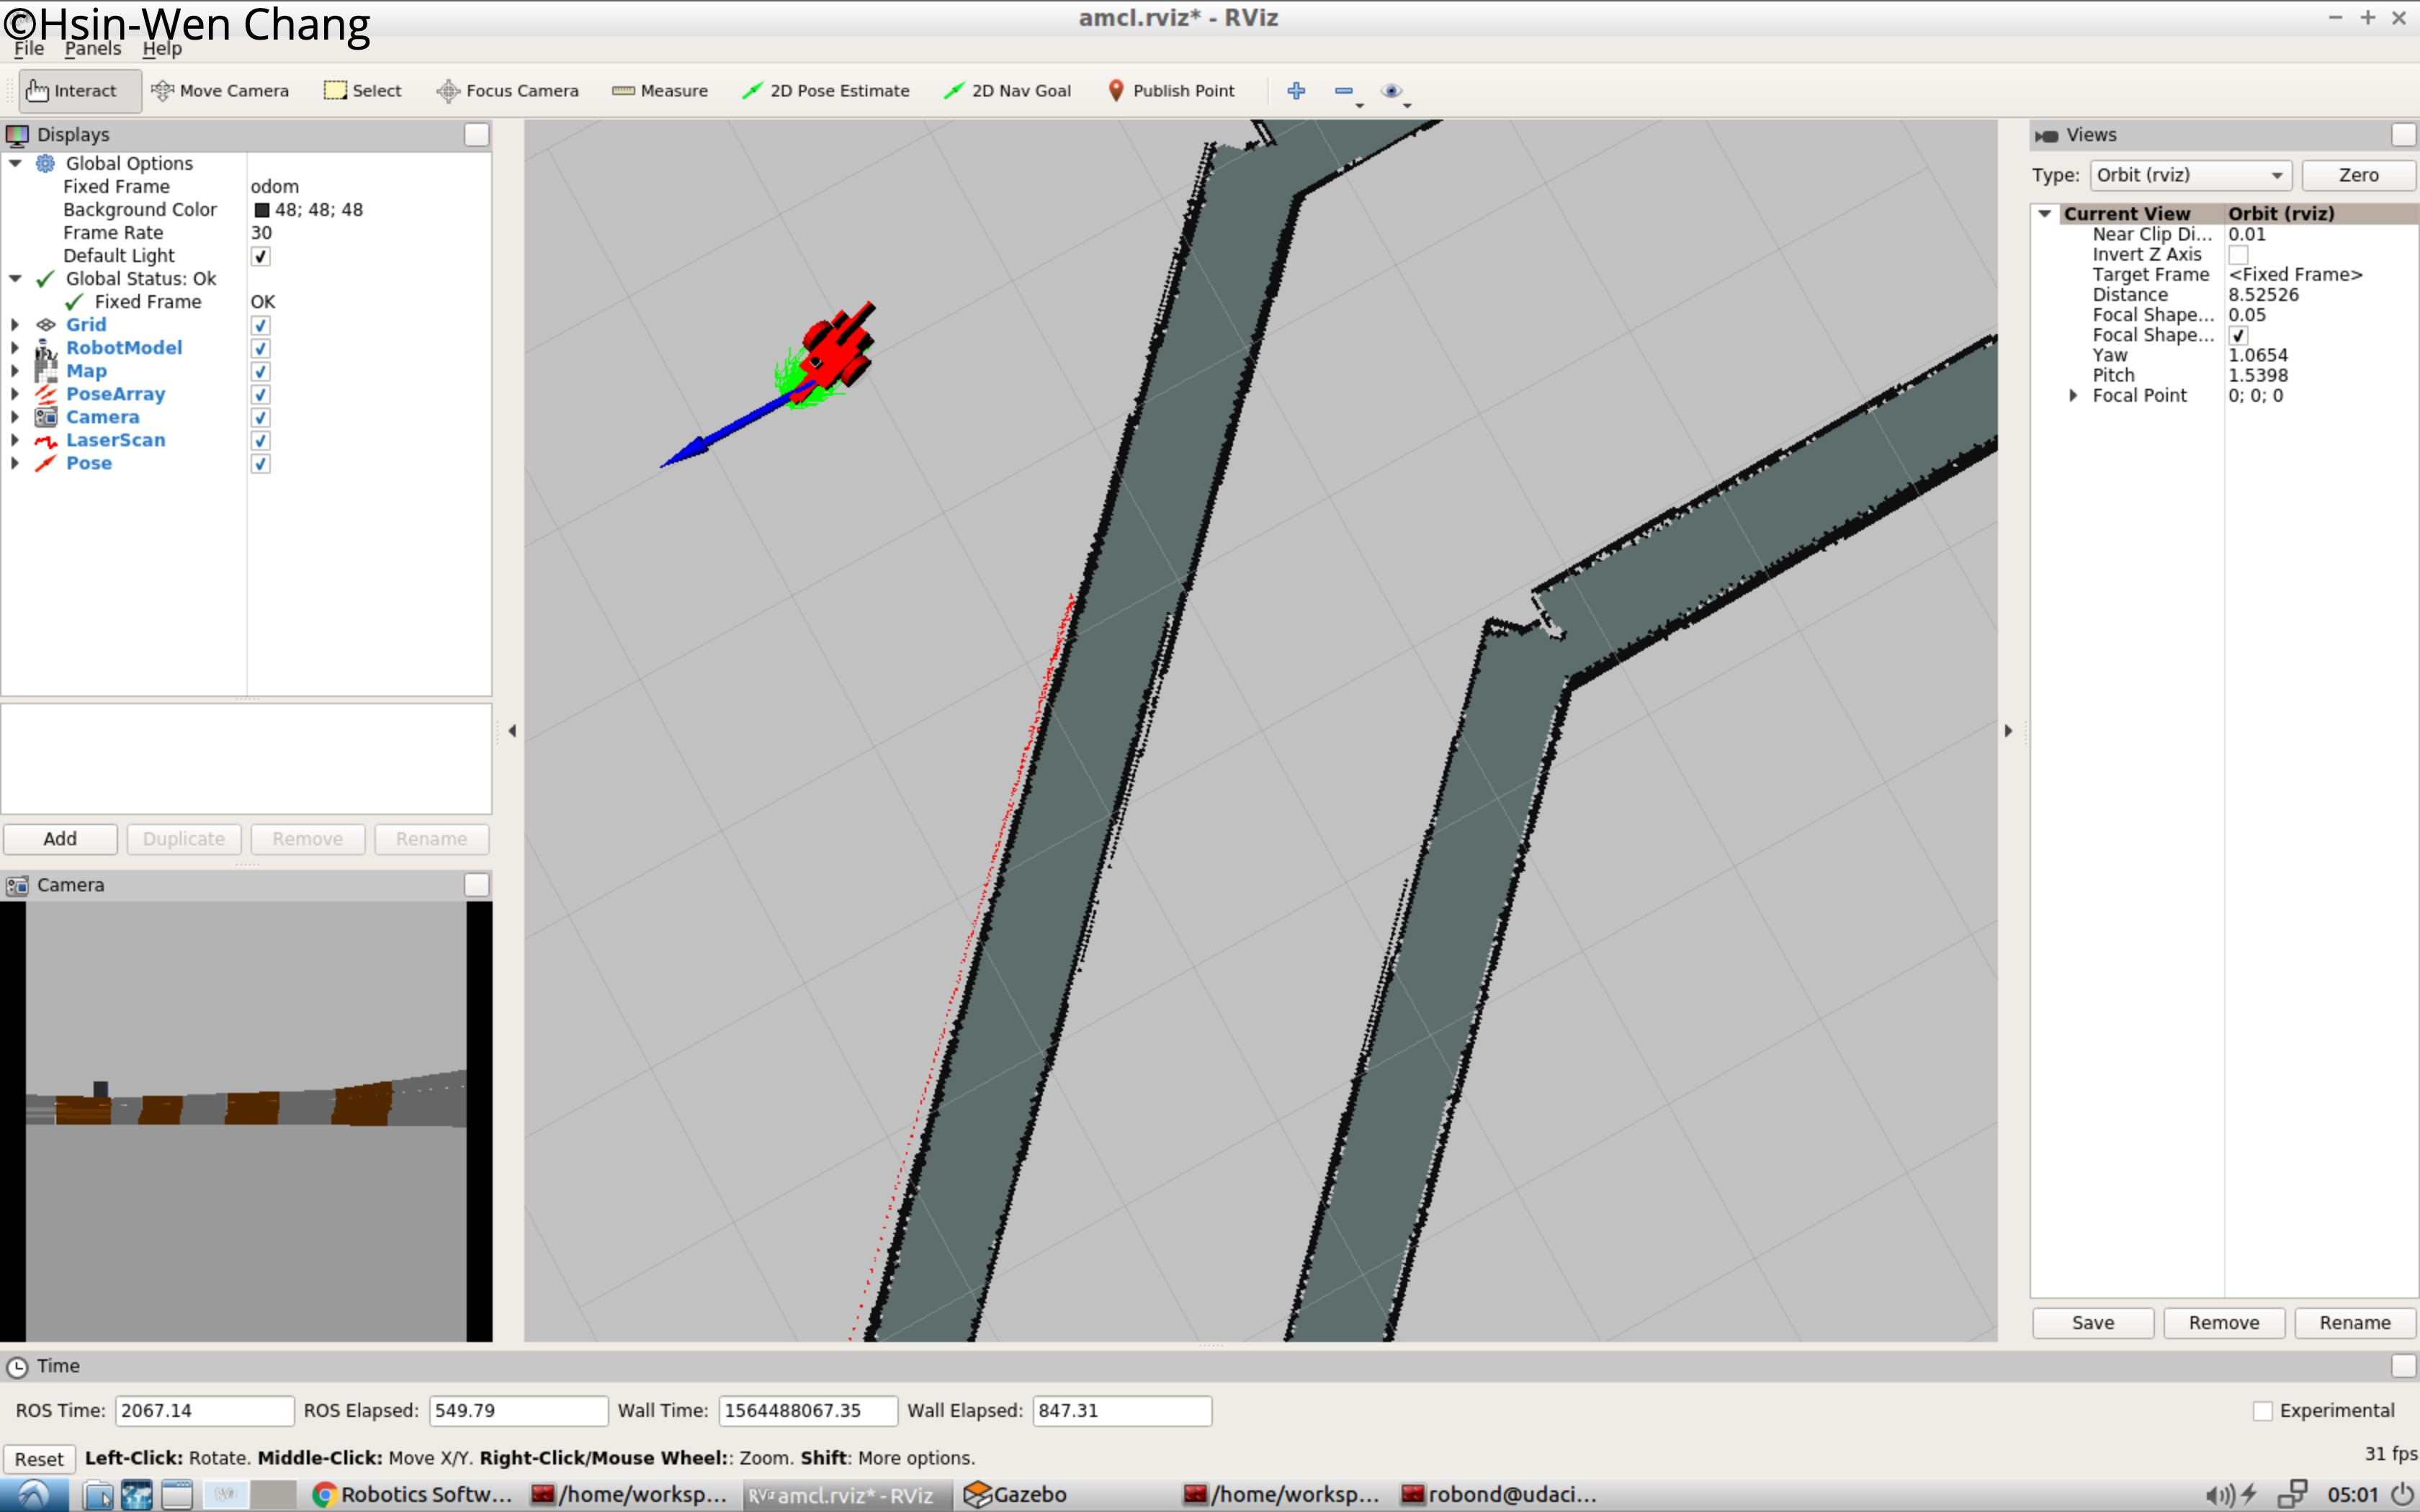
\includegraphics[width=\linewidth]{rvizGoal.png}
      \caption{Hsin bot enter the goal.}
      \label{fig:robot1}
\end{figure}
%example for inserting image
\begin{figure}[thpb]
      \centering
      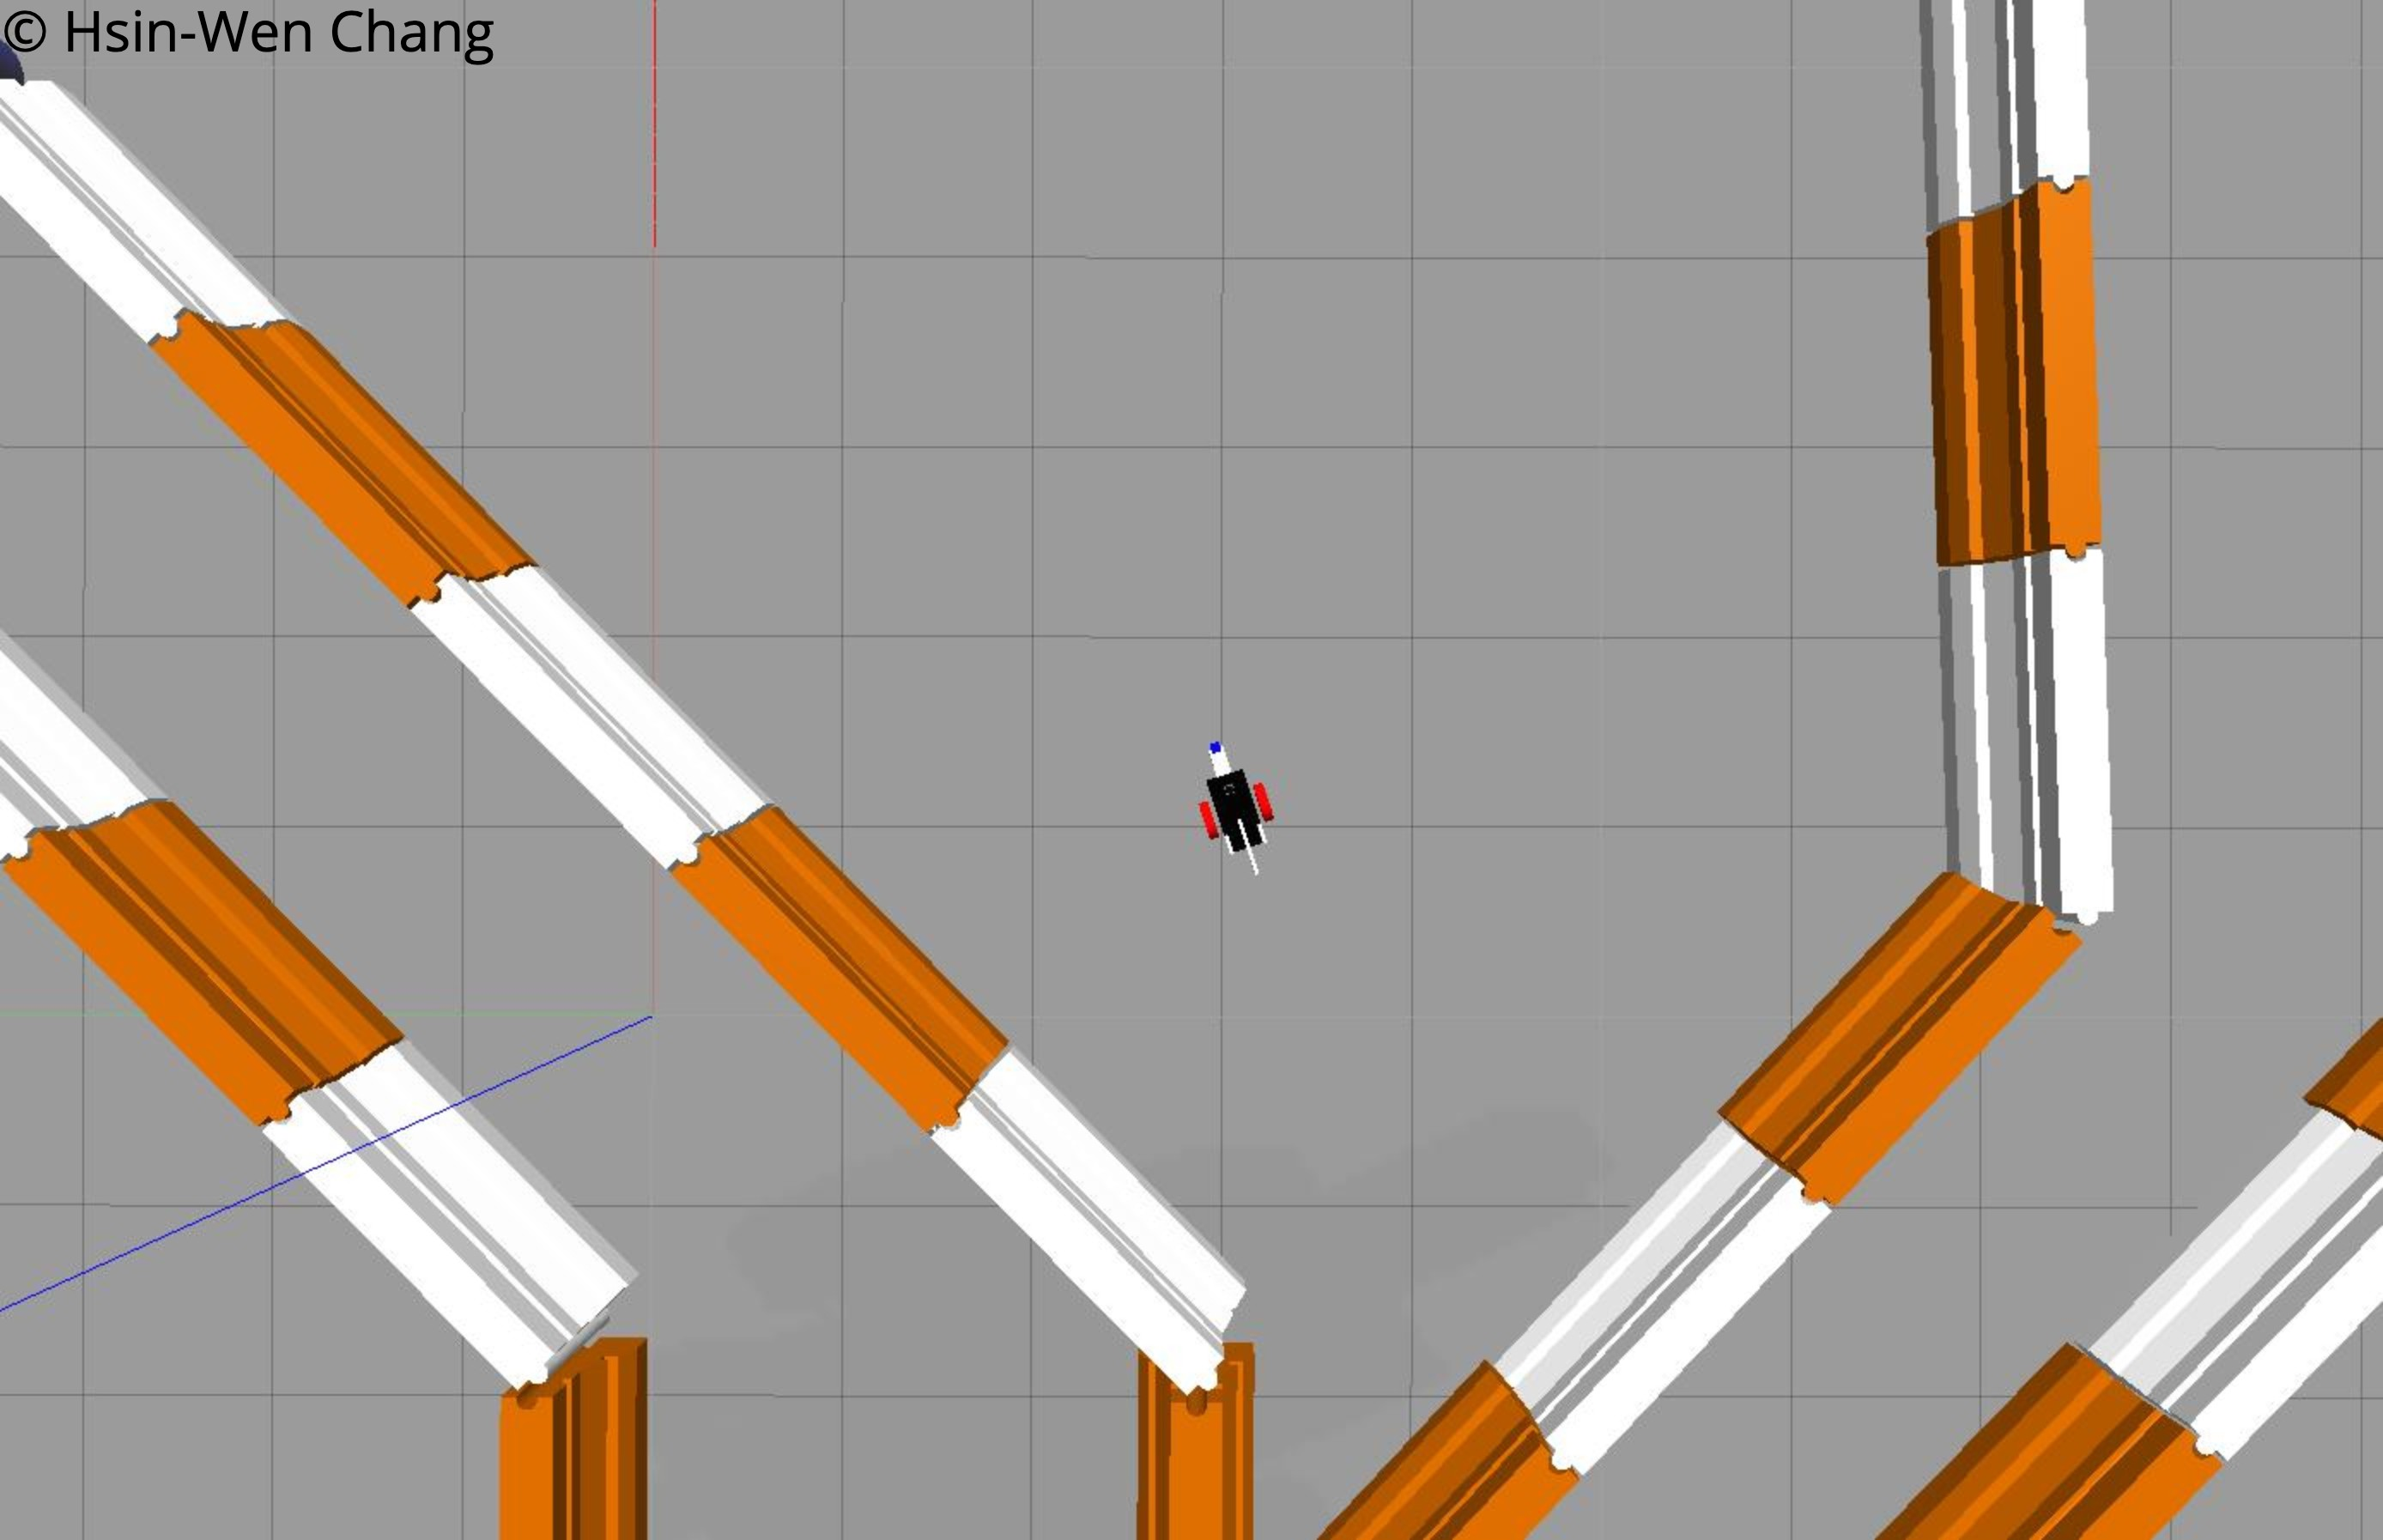
\includegraphics[width=\linewidth]{gazeboGoal.jpg}
      \caption{Hsin bot enter the goal.}
      \label{fig:robot1}
\end{figure}
\subsection{Technical Comparison} % only facts
Discuss the difference of the layout, parameters, performance etc. between the benchmark robot and your robot. It is acceptable for your custom robot to perform worse than the provided robot. The focus is on learning and understanding, not performance. 

\section{Discussion}

 

\subsection{Topics}
\begin{itemize}
\item Which robot performed better?
\item Why it performed better? (opinion)
\item How would you approach the 'Kidnapped Robot' problem?
\item What types of scenario could localization be performed?
\item Where would you use MCL/AMCL in an industry domain?
\end {itemize}

\section{Conclusion / Future work}
This section is intended to summarize your report. Your summary should include a recap of the results, did this project achieve what you attempted, how would you deploy it on hardware and how could this project be applied to commercial products? 
For Future Work, address areas of work that you may not have addressed in your report as possible next steps. This could be due to time constraints, lack of currently developed methods / technology, and areas of application outside of your current implementation. Again, avoid the use of the first-person.

\subsection{Modifications for Improvement}
Examples:
\begin{itemize}
\item Base Dimension
\item Sensor Location
\item Sensor Layout
\item Sensor Amount
\end{itemize}

\subsection{Hardware Deployment}
\begin{enumerate}
\item What would need to be done?
\item Computation time/resource considerations?
\end{enumerate}



\bibliography{bib}
\bibliographystyle{ieeetr}

[1] Robust Monte Carlo Localization for Mobile Robots Sebastian Thrun, Dieter Fox, Wolfram Burgard, and Frank Dellaer, in Artificial Intelligence, Summer 200.

[2] http://wiki.ros.org/amcl#Parameters
\end{document}
